\documentclass[11pt,a4paper]{article}

\usepackage[utf8]{inputenc}
\usepackage[T1]{fontenc}
\usepackage{lmodern}
\usepackage[margin=1in]{geometry}
\usepackage{microtype}
\usepackage{amsmath,amssymb,amsthm}
\usepackage{booktabs}
\usepackage{multirow}
\usepackage{array}
\usepackage[skip=4pt]{caption}
\usepackage{graphicx}
\usepackage{xcolor}
\usepackage{algorithm}
\usepackage{algpseudocode}
\usepackage{listings}
\usepackage{enumitem}
\usepackage[numbers,sort&compress]{natbib}
\usepackage[colorlinks=true,linkcolor=blue!60!black,citecolor=blue!60!black,urlcolor=blue!60!black]{hyperref}

\emergencystretch=2em

\theoremstyle{definition}
\newtheorem{definition}{Definition}

\definecolor{codebg}{RGB}{248,249,250}
\definecolor{codeframe}{RGB}{218,222,226}
\definecolor{diffdel}{RGB}{176,24,42}
\definecolor{diffadd}{RGB}{18,110,62}
\definecolor{codekw}{RGB}{0,70,155}
\definecolor{codecmt}{RGB}{95,105,115}

\lstdefinestyle{sqjcode}{
    backgroundcolor=\color{codebg},
    frame=single,
    rulecolor=\color{codeframe},
    basicstyle=\ttfamily\footnotesize,
    keywordstyle=\color{codekw}\bfseries,
    commentstyle=\color{codecmt}\itshape,
    stringstyle=\color{diffadd},
    breaklines=true,
    breakatwhitespace=false,
    columns=fullflexible,
    keepspaces=true,
    showstringspaces=false,
    aboveskip=0.65em,
    belowskip=0.65em,
    xleftmargin=0.4em,
    xrightmargin=0.4em
}
\lstset{style=sqjcode}

% Auto-generated quantitative macros from data/v2_study_summary_metrics.json (2.3.0-certified)
% Auto-generated by src/generate_v2_latex_and_verify.py (2.3.0-certified) — DO NOT EDIT MANUALLY
\newcommand{\HarnessVer}{\texttt{2.3.0-certified}}
\newcommand{\CtrlTotalOD}{142}
\newcommand{\CtrlTotalValid}{133}
\newcommand{\CtrlTotalUnknown}{9}
\newcommand{\CtrlPyAttempted}{93}
\newcommand{\CtrlPyValid}{90}
\newcommand{\CtrlPyUnknown}{3}
\newcommand{\CtrlPyNonIdempCount}{27}
\newcommand{\CtrlPyNonIdempRepos}{11}
\newcommand{\CtrlJavaAttempted}{49}
\newcommand{\CtrlJavaOrderExact}{49}
\newcommand{\CtrlJavaPhaseKnown}{46}
\newcommand{\CtrlJavaValid}{43}
\newcommand{\CtrlJavaUnknown}{6}
\newcommand{\CtrlJavaNonIdempCount}{5}
\newcommand{\CtrlJavaNonIdempRepos}{2}
\newcommand{\BenchInitAttempted}{208}
\newcommand{\BenchEligible}{203}
\newcommand{\BenchAttritionCount}{5}
\newcommand{\BenchJavaEligible}{110}
\newcommand{\BenchPyEligible}{93}
\newcommand{\BenchJavaID}{61}
\newcommand{\BenchJavaOD}{49}
\newcommand{\BenchPyVictim}{60}
\newcommand{\BenchPyBrittle}{33}
\newcommand{\BenchProjects}{69}
\newcommand{\BenchJavaProjects}{35}
\newcommand{\BenchPyProjects}{34}
\newcommand{\BenchTargetMDetTotal}{4,842}
\newcommand{\BenchTargetMDetMedian}{15}
\newcommand{\BenchPartnerMDetTotal}{1,037}
\newcommand{\BenchODWithPartner}{126}
\newcommand{\BenchODZeroPartner}{16}
\newcommand{\BenchMExtSamples}{177}
\newcommand{\BenchMExtTotal}{3,518}
\newcommand{\PRTotalInstances}{108}
\newcommand{\PRDistinctURLs}{50}
\newcommand{\PREvaluatedClean}{53}
\newcommand{\PRAcceptedTestOnlyWPlus}{16}
\newcommand{\PRLegitTotal}{39}
\newcommand{\PRLegitFalseRejBThree}{1/39}
\newcommand{\PRLegitFalseRejBThreePct}{2.56\%}
\newcommand{\PRLegitFalseRejBThreePlus}{4/39}
\newcommand{\PRLegitFalseRejBThreePlusPct}{10.26\%}
\newcommand{\PRLegitFalseRejMuGuard}{8/39}
\newcommand{\PRLegitFalseRejMuGuardPct}{20.51\%}
\newcommand{\PRShiftSensMuGuard}{9/40 (22.50\%)}
\newcommand{\BOneGptAvail}{75}
\newcommand{\BOneGptWPlus}{33}
\newcommand{\BOneGptEroded}{9}
\newcommand{\BOneGptLeakPct}{27.27\%}
\newcommand{\BOneMagAvail}{13}
\newcommand{\BOneMagWPlus}{4}
\newcommand{\BOneMagEroded}{0}
\newcommand{\BOneMagLeakPct}{0.00\%}
\newcommand{\BOneIpfAvail}{77}
\newcommand{\BOneIpfExcludedMismatch}{3}
\newcommand{\BOneIpfWPlus}{42}
\newcommand{\BOneIpfEroded}{10}
\newcommand{\BOneIpfLeakPct}{23.81\%}
\newcommand{\TaxAppearances}{979}
\newcommand{\TaxUniquePatches}{400}
\newcommand{\TaxDistinctTests}{74}
\newcommand{\TaxDistinctProjects}{27}
\newcommand{\TaxBypassBThree}{396}
\newcommand{\TaxBypassBThreePlus}{335}
\newcommand{\TaxManualN}{60}
\newcommand{\TaxManualGenuineDeg}{44}
\newcommand{\TaxManualRespShift}{12}
\newcommand{\TaxManualLegitArt}{4}
\newcommand{\LatUncachedJavaMutMed}{9.51}
\newcommand{\LatUncachedJavaMutPNinety}{16.56}
\newcommand{\LatUncachedPyMutMed}{3.72}
\newcommand{\LatUncachedPyMutPNinety}{9.88}
\newcommand{\LatBaseCombinedMed}{11.69}
\newcommand{\FlashNElig}{202}
\newcommand{\FlashBZeroWPlusPct}{97.03\%}
\newcommand{\FlashBZeroLeakPct}{19.90\%}
\newcommand{\FlashBZeroSoundPct}{71.29\%}
\newcommand{\FlashBThreeSoundPct}{71.29\%}
\newcommand{\FlashBThreePlusLeakPct}{21.03\%}
\newcommand{\FlashBThreePlusSoundPct}{69.80\%}
\newcommand{\FlashBFourScalarSoundPct}{80.20\%}
\newcommand{\FlashOursSoundPct}{87.62\%}
\newcommand{\FlashOursITTPct}{85.10\%}
\newcommand{\FlashGainVsBThreePlus}{+17.82}
\newcommand{\FlashBZeroExtYsPct}{81.92\%}
\newcommand{\FlashBThreePlusExtYsPct}{79.10\%}
\newcommand{\FlashBFourExtYsPct}{71.75\%}
\newcommand{\FlashOursExtYsPct}{76.27\%}
\newcommand{\FlashBZeroExtYsStressPct}{88.70\%}
\newcommand{\FlashBThreePlusExtYsStressPct}{87.57\%}
\newcommand{\FlashBFourExtYsStressPct}{80.23\%}
\newcommand{\FlashOursExtYsStressPct}{84.75\%}
\newcommand{\FlashOursCondLossPct}{4.43\%}
\newcommand{\FlashRelRedVsBZeroPct}{45.2\%}
\newcommand{\FlashRelRedVsBThreePlusPct}{49.5\%}
\newcommand{\FlashExtGainVsBThreePlus}{-2.82}
\newcommand{\FlashExtStressGainVsBThreePlus}{-2.82}
\newcommand{\FlashBZeroGenLoss}{4}
\newcommand{\FlashBZeroShiftLoss}{8}
\newcommand{\FlashBThreePlusGenLoss}{3}
\newcommand{\FlashBThreePlusShiftLoss}{9}
\newcommand{\FlashBFourGenLoss}{2}
\newcommand{\FlashBFourShiftLoss}{1}
\newcommand{\FlashOursGenLoss}{2}
\newcommand{\FlashOursShiftLoss}{1}
\newcommand{\FlashOursLegitLoss}{4}
\newcommand{\ProNElig}{188}
\newcommand{\ProBZeroWPlusPct}{94.15\%}
\newcommand{\ProBZeroLeakPct}{23.73\%}
\newcommand{\ProBZeroSoundPct}{69.68\%}
\newcommand{\ProBThreeSoundPct}{69.15\%}
\newcommand{\ProBThreePlusLeakPct}{26.92\%}
\newcommand{\ProBThreePlusSoundPct}{68.09\%}
\newcommand{\ProBFourScalarSoundPct}{78.19\%}
\newcommand{\ProOursSoundPct}{85.11\%}
\newcommand{\ProOursITTPct}{76.92\%}
\newcommand{\ProGainVsBThreePlus}{+17.02}
\newcommand{\ProBZeroExtYsPct}{72.32\%}
\newcommand{\ProBThreePlusExtYsPct}{72.88\%}
\newcommand{\ProBFourExtYsPct}{66.67\%}
\newcommand{\ProOursExtYsPct}{71.19\%}
\newcommand{\ProBZeroExtYsStressPct}{77.97\%}
\newcommand{\ProBThreePlusExtYsStressPct}{79.10\%}
\newcommand{\ProBFourExtYsStressPct}{72.88\%}
\newcommand{\ProOursExtYsStressPct}{77.40\%}
\newcommand{\ProOursCondLossPct}{4.83\%}
\newcommand{\ProRelRedVsBZeroPct}{49.4\%}
\newcommand{\ProRelRedVsBThreePlusPct}{57.3\%}
\newcommand{\ProExtGainVsBThreePlus}{-1.69}
\newcommand{\ProExtStressGainVsBThreePlus}{-1.69}
\newcommand{\ProBZeroGenLoss}{3}
\newcommand{\ProBZeroShiftLoss}{9}
\newcommand{\ProBThreePlusGenLoss}{6}
\newcommand{\ProBThreePlusShiftLoss}{9}
\newcommand{\ProBFourGenLoss}{2}
\newcommand{\ProBFourShiftLoss}{0}
\newcommand{\ProOursGenLoss}{3}
\newcommand{\ProOursShiftLoss}{2}
\newcommand{\ProOursLegitLoss}{2}
\newcommand{\QwenNElig}{203}
\newcommand{\QwenBZeroWPlusPct}{88.67\%}
\newcommand{\QwenBZeroLeakPct}{20.56\%}
\newcommand{\QwenBZeroSoundPct}{65.02\%}
\newcommand{\QwenBThreeSoundPct}{67.00\%}
\newcommand{\QwenBThreePlusLeakPct}{22.29\%}
\newcommand{\QwenBThreePlusSoundPct}{63.05\%}
\newcommand{\QwenBFourScalarSoundPct}{75.37\%}
\newcommand{\QwenOursSoundPct}{79.31\%}
\newcommand{\QwenOursITTPct}{77.40\%}
\newcommand{\QwenGainVsBThreePlus}{+16.26}
\newcommand{\QwenBZeroExtYsPct}{72.32\%}
\newcommand{\QwenBThreePlusExtYsPct}{71.75\%}
\newcommand{\QwenBFourExtYsPct}{67.23\%}
\newcommand{\QwenOursExtYsPct}{70.06\%}
\newcommand{\QwenBZeroExtYsStressPct}{77.97\%}
\newcommand{\QwenBThreePlusExtYsStressPct}{79.66\%}
\newcommand{\QwenBFourExtYsStressPct}{75.71\%}
\newcommand{\QwenOursExtYsStressPct}{78.53\%}
\newcommand{\QwenOursCondLossPct}{4.11\%}
\newcommand{\QwenRelRedVsBZeroPct}{64.8\%}
\newcommand{\QwenRelRedVsBThreePlusPct}{59.4\%}
\newcommand{\QwenExtGainVsBThreePlus}{-1.69}
\newcommand{\QwenExtStressGainVsBThreePlus}{-1.13}
\newcommand{\QwenBZeroGenLoss}{7}
\newcommand{\QwenBZeroShiftLoss}{9}
\newcommand{\QwenBThreePlusGenLoss}{6}
\newcommand{\QwenBThreePlusShiftLoss}{8}
\newcommand{\QwenBFourGenLoss}{2}
\newcommand{\QwenBFourShiftLoss}{0}
\newcommand{\QwenOursGenLoss}{2}
\newcommand{\QwenOursShiftLoss}{0}
\newcommand{\QwenOursLegitLoss}{4}
\newcommand{\ForkTotal}{128}
\newcommand{\ForkTotalATwo}{116}
\newcommand{\ForkTests}{61}
\newcommand{\ForkProjects}{20}
\newcommand{\ForkFlashNzRepos}{7}
\newcommand{\ForkProNzRepos}{5}
\newcommand{\ForkQwenNzRepos}{6}
\newcommand{\ForkAOneCount}{55}
\newcommand{\ForkAOnePct}{42.97\%}
\newcommand{\ForkATwoCount}{42}
\newcommand{\ForkATwoPct}{36.21\%}
\newcommand{\ForkAThreeCount}{91}
\newcommand{\ForkAThreePct}{71.09\%}
\newcommand{\ForkDiffAThreeVsAOne}{+28.12}
\newcommand{\ForkCIAThreeVsAOne}{[+11.84, +43.56]}
\newcommand{\ForkPClusterAThreeVsAOne}{0.0049}
\newcommand{\ForkEqModelDiff}{+27.88}
\newcommand{\ForkEqModelCI}{[+11.91, +43.60]}
\newcommand{\ForkEqModelP}{0.0039}
\newcommand{\ForkDiffAThreeVsATwo}{+37.07}
\newcommand{\ForkPClusterAThreeVsATwo}{0.0005}
\newcommand{\ForkCharDiffMed}{120}
\newcommand{\ForkCharDiffMax}{1137}


\title{\textbf{Stabilization via Oracle Erosion: An Empirical Audit and Local Mutation Gate for Flaky Test Repair}}

\author{
  Zhijie Li$^{1}$, Ketong Liu$^{1}$, Shaoyang Xu$^{1}$, Shibo Meng$^{1}$, Feiran Gao$^{2}$, and Yuli Zhao$^{1*}$ \\[0.55em]
  \small $^{1}$Software College, Northeastern University, Shenyang, China \\
  \small $^{2}$School of Computer Science and Technology, Beijing Institute of Technology, Beijing, China \\[0.35em]
  \footnotesize \textit{Emails:} \href{mailto:lizhijie@mails.neu.edu.cn}{lizhijie@mails.neu.edu.cn}, \href{mailto:liuketong@mails.neu.edu.cn}{liuketong@mails.neu.edu.cn}, \href{mailto:xusy3@mails.neu.edu.cn}{xusy3@mails.neu.edu.cn}, \\
  \footnotesize \href{mailto:mengsb1@mails.neu.edu.cn}{mengsb1@mails.neu.edu.cn}, \href{mailto:3120260997@bit.edu.cn}{3120260997@bit.edu.cn}, \href{mailto:zhaoyl@swc.neu.edu.cn}{zhaoyl@swc.neu.edu.cn} ($^{*}$Corresponding author)
}
\date{}

\begin{document}
\maketitle

\begin{abstract}
Automated flaky test repair tools increasingly combine context localization with large language models to remove intermittent continuous integration failures. However, nearly every pipeline accepts a candidate patch once it compiles, passes rerun schedules, and keeps its assertion statements. Because test repair edits the test oracle and fixture themselves, optimizing solely for green runs invites \emph{Stabilization via Oracle Erosion}. Eroded tests turn permanently green while losing their ability to catch future production faults. We audit 203 flaky Java and Python tests, comparing historical repair artifacts, developer pull requests, and five modern language models. Roughly one in five to one in four stabilization-passing patches from prior tools and unconstrained models silently drops baseline fault-detection obligations. Even a strengthened structural static guard fails to block over four-fifths of eroded patches because semantic shifts evade syntax checks. We introduce \textsc{MuGuard-Flake}, a fail-closed local mutation gate that verifies modified tests and their shared-state partners before merging a repair. It eliminates erosion during repair, raises operational sound-fix yield, and cuts unseen fault-detection loss among accepted patches by 45\% to 65\%, running in seconds per candidate. Strict gating is not free: conservative abstention leaves overall end-to-end held-out yield statistically inconclusive and rejects 20.5\% of legitimate developer pull requests. In a controlled feedback comparison, concrete surviving-mutant witnesses recover far more eroded repairs than bare numeric counts (71\% versus 43\%).
\end{abstract}

\medskip
\noindent\textbf{Keywords:} Flaky test repair $\cdot$ Oracle erosion $\cdot$ Mutation testing $\cdot$ Large language models $\cdot$ Continuous integration quality gates $\cdot$ Empirical software engineering

\section{Introduction}
\label{sec:intro}

Flaky tests pass and fail unpredictably on the same commit of production code. They erode developer trust in continuous integration (CI), stall release pipelines, and mask genuine regressions~\cite{luo2014empirical,parry2021survey}. Among non-concurrency root causes, two categories dominate automated flaky test repair across Java and Python suites. \emph{Implementation-Dependent} (ID) tests rely on unspecified iteration orders in hash collections, reflection APIs, or JSON serializers~\cite{gyori2016nondex}. \emph{Order-Dependent} (OD) tests depend on shared mutable state polluted or initialized by earlier tests~\cite{lam2019idflakies,shi2019ifixflakies,wang2022ipflakies}.

Automated repair for these tests has advanced rapidly from suite search and syntactic templates, such as \textsc{iFixFlakies}~\cite{shi2019ifixflakies}, \textsc{DexFix}~\cite{zhang2021dexfix}, and \textsc{iPFlakies}~\cite{wang2022ipflakies}, to iterative large language model (LLM) agents including \textsc{FlakyDoctor}~\cite{chen2024flakydoctor} and industrial repair pipelines~\cite{rastenis2026autocover,leunig2026perl}. Across these systems, however, patch acceptance remains governed by a \emph{single-sided stabilization validator}. Once a candidate edit compiles, passes \textsc{NonDex}~\cite{gyori2016nondex} or order-schedule reruns, and keeps its assertion statements intact, the pipeline accepts the patch and stops.

\paragraph{Stabilization via Oracle Erosion.}
Optimizing solely for execution stability creates a subtle quality hazard that we call \emph{Stabilization via Oracle Erosion}. In automated program repair on production code~\cite{qi2015kali,smith2015cure}, an external test suite constrains candidate edits and exposes broken functionality. Flaky test repair lacks that safeguard because it modifies the test oracle and fixture themselves. A concrete example from Apache Commons Lang illustrates the mechanism. In \texttt{ToStringBuilderTest}, an LLM repair replaced a strict reflection-output check with Java's single-argument \texttt{split(",")} to remove iteration-order sensitivity. That patch passed every stability rerun, but single-argument splitting silently drops trailing empty tokens and left eight production faults in \texttt{ToStringStyle} undetected. Once merged, an eroded test turns permanently green and raises no CI alarm.

Warning signs of this hazard have appeared across separate lines of software quality research. \textsc{TestBoost}~\cite{li2024testboost} found that nearly a third of fixture-transformed test classes lost mutation-killing ability despite passing order checks. In this journal, Leunig and Petersen~\cite{leunig2026perl} reported that LLM-driven test repair at IBM frequently diluted assertion specificity behind green pass rates, and Bludau and Pretschner~\cite{bludau2026szz} showed how noisy evaluation proxies distort reported effectiveness. Four empirical questions remain unanswered. First, once we control for flaky mutants~\cite{parry2026flimsiness} and verify actual patch provenance, how often does silent oracle erosion occur across historical tools and modern LLMs, and what false-rejection boundaries emerge on developer pull requests? Second, which edit mechanisms drive erosion, and why do stronger static structural guards fail to block them? Third, how does a fail-closed, test-scoped mutation gate balance operational safety against abstention and held-out yield, and how much recovery do localized witnesses add over bare numeric counts? Fourth, what uncached probing times, abstention causes, and mutant-subset trade-offs arise in practice?

\paragraph{Cross-Language Study and MuGuard-Flake.}
To measure erosion without grading a gate on the same mutants it optimizes against, we build a dual-language benchmark of $\BenchEligible$ flaky tests across $\BenchProjects$ Java and Python repositories. Each baseline fault obligation is verified across repeated clean runs in the test's dynamically executed focal scope, alongside separate obligations for shared-state partner tests whenever order-dependent edits touch fixtures (Section~\ref{sec:construct}). Before inspecting any candidate repair, we freeze $\BenchMExtTotal$ disjoint held-out faults and independent stability schedules to evaluate generalization cleanly. We also collect and manually audit $\PRTotalInstances$ PR-linked Java test instances to measure false rejections on legitimate human fixes.

Building on this benchmark, we design \textsc{MuGuard-Flake}, a fail-closed local mutation gate inspired by error-controlling LLM testing gates~\cite{salva2026nltestrunner} and diagnostic feedback studies~\cite{zhang2026typerepair} (Section~\ref{sec:methodology}). Any candidate failing compilation or stability reruns short-circuits immediately before mutation probing. For stabilized patches, \textsc{MuGuard-Flake} maps every edited test and affected partner scope, probes baseline focal obligations in seconds, and feeds up to four surviving-mutant witnesses back to the model on erosion retries. If a five-round budget expires without an obligation-preserving fix, the gate abstains and hands those witnesses to maintainers instead of merging a weakened test.

\paragraph{Contributions.}
This paper makes four empirical and engineering contributions to software quality assurance:
\begin{enumerate}
    \item \emph{Cross-Language Erosion Audit and Pull-Request Boundaries.} Across $\BenchEligible$ flaky tests, historical repair tools, and five LLMs from four vendors, roughly one in five to one in four stabilization-passing patches silently drops baseline obligations. Checking both target and partner scope across manually reviewed developer pull requests establishes a \PRLegitFalseRejMuGuardPct{} false-rejection rate on legitimate repairs alongside subtle weakening patches missed by standard mutators.
    \item \emph{Edit-Mechanism Taxonomy and Static-Guard Blind Spots.} Auditing \TaxUniquePatches{} unique eroded patches alongside a \TaxManualN-patch manual review explains why over four-fifths of eroded patches bypass an enhanced static structural guard. Precondition shifts, delimiter normalizations, partner-scope edits, and focal call bypasses evade syntactic rules, and static heuristics even reduce sound-fix yield on an out-of-sample model.
    \item \emph{Fail-Closed Mutation Gating and Witness Isolation.} \textsc{MuGuard-Flake} eliminates erosion during repair across all five models, raises operational sound-fix yield by 12 to 18 percentage points over static guards on multi-round backbones, and cuts unseen held-out fault loss among accepted patches by 45\% to 65\%. Conservative abstention leaves overall end-to-end held-out yield statistically inconclusive, whereas a controlled feedback comparison shows that concrete surviving-mutant witnesses recover far more eroded repairs than bare numeric counts.
    \item \emph{Uncached Probing Budgets and Open Replication Package.} Even without caching, focal mutation probing requires under ten seconds median in Java and under four seconds in Python, whereas model reasoning dominates end-to-end latency. We diagnose why abstentions occur, quantify the safety--cost trade-off of sampling smaller mutant subsets, and release all manifests, regression tests, execution traces, and verification scripts.
\end{enumerate}

The remainder of this paper reviews related work (Section~\ref{sec:related}), formalizes oracle erosion and external validation (Section~\ref{sec:construct}), details \textsc{MuGuard-Flake} (Section~\ref{sec:methodology}), presents our experimental design and results (Sections~\ref{sec:design}--\ref{sec:results}), and discusses deployment boundaries, examines validity threats, and concludes (Sections~\ref{sec:discussion}--\ref{sec:conclusion}).

\section{Background and Related Work}
\label{sec:related}

Prior flaky-test repair systems optimize stability without checking fault detection inside the repair loop, whereas test-evolution and empirical-methodology research explains why proxy checks silently erode oracle strength. Table~\ref{tab:related_boundary} positions \textsc{MuGuard-Flake} across three intersecting threads: automated flaky-test stabilization, oracle quality and test flimsiness, and bias-aware, safety-gated testing.

\begin{table*}[t]
\centering
\caption{Methodological positioning of \textsc{MuGuard-Flake} relative to representative flaky test repair, test transformation, and quality-assurance studies.}
\label{tab:related_boundary}
\scriptsize
\setlength{\tabcolsep}{4pt}
\begin{tabular}{>{\raggedright\arraybackslash}p{2.7cm}>{\raggedright\arraybackslash}p{1.8cm}>{\raggedright\arraybackslash}p{4.0cm}>{\raggedright\arraybackslash}p{5.6cm}}
\toprule
Study or System & Venue & Primary Validation Criterion & Limitation or Methodological Role \\
\midrule
\textsc{DexFix}~\cite{zhang2021dexfix} & ICSE 2021 & Template rules and \textsc{NonDex} reruns & Permissive comparators such as non-strict JSON equality mask extraneous or corrupted fields. \\
\textsc{iPFlakies}~\cite{wang2022ipflakies} & ICSE-Comp.\ 2022 & Polluter search and order reruns in Python & Spliced cleaners or minimal setup calls can drop preconditions needed by focal assertions. \\
\textsc{FlakyDoctor}~\cite{chen2024flakydoctor} & ISSTA 2024 & Neurosymbolic localization and LLM reruns & No in-loop fault-detection check verifies whether stabilized patches retain regression sensitivity. \\
\textsc{TestBoost}~\cite{li2024testboost} & ASE 2024 & Fixture-sharing transform and post-hoc mutation audit & Shows 30.7\% of transformed classes lose mutation kills, without an automated repair gate. \\
\textsc{Test Flimsiness}~\cite{parry2026flimsiness} & ICSE 2026 & Multi-run mutation testing for flaky kills & Characterizes noisy kills; we counter flimsiness by requiring consistent kills across repeated isolated runs. \\
Leunig \& Petersen~\cite{leunig2026perl} & SQJ 2026 & Industrial LLM test-repair audit at IBM & Shows green execution conceals assertion dilution; motivates executable conservation gates. \\
Bludau \& Pretschner~\cite{bludau2026szz} & SQJ 2026 & Ground-truth swap for proxy evaluation bias & Motivates measuring the inflation gap between stabilization, in-loop preservation, and external fault retention. \\
Zhang et al.~\cite{zhang2026typerepair} & SQJ 2026 & Present, absent, and mismatched diagnostic control & Inspires our controlled contrast of absent, misleading, and accurate witness feedback. \\
Salva~\cite{salva2026nltestrunner} & SQJ 2026 & False-acceptance vs.\ false-rejection control & Inspires our fail-closed three-state CI gate and explicit pull-request false-rejection audit. \\
\midrule
\textbf{MuGuard-Flake} & \textbf{This Paper} & \textbf{Fail-closed stability and dual-role focal mutation gate, localized witness retry, and witness-backed abstention} & \textbf{Benchmarks against static, dynamic coverage, and cross-vendor LLM-judge gates across five LLMs, historical tools, and developer PRs.} \\
\bottomrule
\end{tabular}
\end{table*}

\subsection{Root Causes and Automated Repair of Flaky Tests}

Intermittent test failures weaken regression signaling in CI by breaking the link between test verdicts and code changes~\cite{luo2014empirical,lam2020lifecycle,parry2021survey}. Empirical taxonomies highlight two context-sensitive categories as primary targets for automated repair~\cite{lam2019idflakies,gyori2016nondex,wang2022ipflakies}. Implementation-Dependent (ID) tests rely on unspecified library behavior, such as hash-map iteration order, reflection ordering, or unordered JSON serialization~\cite{gyori2016nondex,zhang2021dexfix}; \textsc{NonDex} exposes them by permuting internal data structures across seeds. Order-Dependent (OD) tests depend on shared mutable state left behind by earlier tests, such as static fields, singletons, system properties, or files~\cite{lam2019idflakies,shi2019ifixflakies,wang2022ipflakies}. Order-dependent tests split into \emph{victims}, which pass in isolation but fail after a state-polluting test, and \emph{brittles}, which fail in isolation unless preceded by a state-setter test~\cite{shi2019ifixflakies,wang2022ipflakies}.

Automated repair progressed from suite search and syntax templates to LLM agents. \textsc{iFixFlakies}~\cite{shi2019ifixflakies} and \textsc{iPFlakies}~\cite{wang2022ipflakies} mine cleaner or helper statements from the test suite and splice them into order-dependent tests. \textsc{DexFix}~\cite{zhang2021dexfix} applies syntax templates, such as switching unordered sets to linked variants or relaxing exact JSON equality to non-strict mode, to fix implementation-dependent tests. More recently, \textsc{FlakyDoctor}~\cite{chen2024flakydoctor} pairs dynamic localization with iterative LLM repair under rerun validation, and industrial systems such as \textsc{AutoCover}~\cite{rastenis2026autocover} and database flakiness repair pipelines~\cite{berndt2026dbms} adopt similar generate-and-rerun loops.

Across these pipelines, acceptance remains single-sided: any candidate that compiles and passes the stability rerun suite is accepted. Even in template repair, Zhang et al.~\cite{zhang2021dexfix} noted that relaxing JSON checks to ignore key order can admit extra or corrupted fields. Yet neither \textsc{FlakyDoctor}~\cite{chen2024flakydoctor} nor suite-search tools verify inside the repair loop whether a stabilized test preserves its original fault-detection power.

\subsection{Patch Overfitting, Oracle Quality, and Test Flimsiness}

Oracle erosion in flaky test repair is a sharper form of patch overfitting in automated program repair (APR). In production APR, generate-and-validate loops often emit plausible patches that pass weak test suites by deleting behavior or bypassing faulty paths~\cite{qi2015kali,smith2015cure}. Test repair faces a deeper structural asymmetry~\cite{barr2015oracle,daniel2009reassert,li2019trip,rahman2025utfix}. Whereas production APR leaves the test suite intact as an external referee, flaky test repair edits the test oracle and fixture themselves. Once an assertion is weakened, CI reports a permanently green build with no failure signal.

Prior test-evolution studies confirm that automated test edits can silently mask regressions, yet existing checks leave an online verification gap. Early tools such as \textsc{ReAssert}~\cite{daniel2009reassert} risked hiding bugs by rewriting expected values from live runs. More recently, \textsc{TestBoost}~\cite{li2024testboost} found post hoc that 30.7\% of fixture-transformed classes lost mutation kills, and change-aware repair tools~\cite{li2019trip,rahman2025utfix} target evolving production code rather than flaky-test stabilization. Dynamic coverage and static diff review also fall short as online guards. Checked Coverage~\cite{schuler2013checked} demonstrated that statement and branch coverage record line execution rather than whether assertions inspect computed state, and standalone LLM judges score diff plausibility without observing which production branches stop influencing test verdicts.

Evaluating test edits with mutation testing builds on extensive evidence linking mutant kills to real fault detection~\cite{just2014mutants,papadakis2019mutation}, yet introduces its own measurement hazards. Automatically generated suites are frequently flaky~\cite{gruber2024generated}, and mutation scores in LLM-generated suites shift with granularity and code version~\cite{zhao2026correlation}. Most directly, Parry et al.~\cite{parry2026flimsiness} formalized \emph{Test Flimsiness}: mutating production code can trigger intermittent failures in otherwise passing tests, causing single-run mutation testing to credit chance failures as genuine kills. To rule out flimsy kills, Section~\ref{sec:construct} retains only baseline mutants that fail deterministically in the target test across repeated isolated runs, and cross-checks accepted repairs on disjoint held-out faults.

\subsection{Proxy Bias, Diagnostic Controls, and Safety-Gated Testing}

Sound evaluation of repair gates must confront two recurring validity threats: green pass rates that conceal weakened assertions and proxy metrics that conflate distinct quality dimensions. In an industrial study at IBM, Leunig and Petersen~\cite{leunig2026perl} showed that pass rates hide assertion dilution during iterative LLM test repair, and Bludau and Pretschner~\cite{bludau2026szz} demonstrated how noisy proxy labels distort empirical rankings. Following those lessons, we separate stability, in-loop fault preservation, independent held-out fault detection, and semantic erosion types instead of collapsing them into a single repair rate.

Turning diagnosis into a practical CI gate also requires testing whether error feedback truly drives repair gains and measuring the cost of conservatism. Adopting the diagnostic-control logic of Zhang et al.~\cite{zhang2026typerepair}, who contrasted accurate, absent, and mismatched error signals in LLM repair, we test whether localized surviving-mutant feedback outperforms bare numeric counts or misleading hints. On the deployment side, Salva~\cite{salva2026nltestrunner} framed LLM testing agents around explicit retry-and-abstention control of false acceptances versus false rejections. \textsc{MuGuard-Flake} unifies these principles in a fail-closed CI merge gate whose false-rejection rate, external fault-detection benefit, and runtime overhead we measure end to end. Closing the gaps across these three threads first requires formalizing oracle erosion and non-circular external validation, which we turn to next.

\section{Problem Formulation: Stabilization via Oracle Erosion}
\label{sec:construct}

To ground both our empirical audit and our repair gate without circularity, we formalize flaky test stabilization, attributed fault obligations, partner-scope conservation, and disjoint external validation. The box below summarizes core notation; language-specific instrumentation mechanics appear in Section~\ref{sec:impl}.

\medskip
\noindent\fbox{\parbox{0.97\textwidth}{\scriptsize\setlength{\tabcolsep}{2.5pt}
\textbf{Core Notation and Metric Quick Reference}\\[0.2em]
\begin{tabular}{@{}p{0.14\textwidth}p{0.31\textwidth}@{\hspace{0.015\textwidth}}p{0.15\textwidth}p{0.31\textwidth}@{}}
$P_0, T_{\text{orig}}, T_{\text{part}}$ & Frozen production code, target test, and OD partner & $\mathcal{O}_{\text{joint}}, R_{\text{joint}}$ & Role-tagged target-and-partner obligation union and retention \\
$e_0, e_{\text{iso}}$ & Clean baseline schedule and isolated standalone check & $\Delta_{\text{inf}}$ & Proxy Inflation Gap ($\text{Pass@}W^+\% - \text{SoundFix}\%$) \\
$W^+, W^+_{\text{heldout}}$ & In-loop and disjoint held-out stability schedules & $M_{\text{ext-op}}, M_{\text{ext-inst}}$ & Disjoint held-out mutants (unseen operators and overflow sites) \\
$M_{\text{focal}}, M_{\text{det}}$ & Covered focal mutants and $3/3$ attributed kill baseline & $Y_s^{\text{strict}}, Y_s^{\text{stress}}$ & Fixed-cohort end-to-end held-out yield (strict vs.\ stress) \\
\end{tabular}
}}
\medskip

\subsection{Clean Reference Execution (\texorpdfstring{$e_0$}{e0}) and Stabilization Schedules (\texorpdfstring{$W^+$}{W+})}

Let $P_0$ denote the unmodified production code at a frozen benchmark commit, and let $T_{\text{orig}}$ denote a target flaky test in suite $\mathcal{T}$, paired with partner test $T_{\text{part}}$ when order-dependent. Running test $T$ against program $P$ under schedule $e$ records the executed test case, lifecycle phase (setup, call, or teardown), exception type, and final status. Each run resolves to pass, call failure, setup or infrastructure error, skip, timeout, or compile error.

\begin{definition}[Clean Reference Configuration $e_0$]
\label{def:e0}
For a flaky test $T_{\text{orig}}$, its \emph{clean reference configuration} $e_0$ is the canonical schedule under which $T_{\text{orig}}$ passes reliably on unmodified production code $P_0$:
\begin{itemize}[nosep]
    \item For an ID or OD-victim test, $e_0$ runs $T_{\text{orig}}$ alone in a fresh process with default library settings and random-order plugins disabled.
    \item For an OD-brittle test paired with its minimal state-setter $T_{\text{set}}$, $e_0$ runs $\langle T_{\text{set}}, T_{\text{orig}} \rangle$ in a fresh process.
\end{itemize}
To exclude timing or external-I/O nondeterminism, $T_{\text{orig}}$ must pass $e_0$ across five consecutive independent runs before entering the cohort.
\end{definition}

\begin{definition}[In-Loop Stabilization $W^+$ and Held-Out Schedules $W^+_{\text{heldout}}$]
\label{def:w_plus}
Let $W^+(T_{\text{orig}})$ denote the specification-preserving perturbations checked inside the repair loop, and let $W^+_{\text{heldout}}(T_{\text{orig}})$ denote a disjoint held-out stability check:
\begin{itemize}[nosep]
    \item \emph{Java ID tests.} In-loop $W^+$ runs five \textsc{NonDex}~\cite{gyori2016nondex} permutations. Held-out $W^+_{\text{heldout}}$ runs five disjoint deterministic seeds never seen during repair.
    \item \emph{Java and Python OD tests.} In-loop $W^+$ executes three fresh-process schedules: standalone $\langle T \rangle$, coupled $\langle T_{\text{part}}, T \rangle$, and reverse $\langle T, T_{\text{part}} \rangle$. Held-out $W^+_{\text{heldout}}$ repeats each schedule twice and adds one single-lifecycle repeated-pollution run $\langle p_1, p_2, \text{target} \rangle = \langle T_{\text{part}}, T_{\text{part}}, T \rangle$.
\end{itemize}
A candidate patch $T'$ achieves stabilization (\emph{Pass@$W^+$}) if it compiles cleanly and passes every schedule in $W^+(T_{\text{orig}})$ with zero failures, errors, or skipped tests.
\end{definition}

The repeated-pollution schedule tests whether state leaks across back-to-back partner runs in one lifecycle by tracking slots $p_1$, $p_2$, and target. Under our primary strict rule, all three slots must pass every lifecycle phase. Because some unmodified partner tests are non-idempotent when invoked twice, we also run unmodified-repository controls for every order-dependent test. Our secondary stress-relaxed check excuses a $p_2$ call failure only when $T_{\text{part}}$ is untouched, setup and teardown pass cleanly, and an unmodified control reproduces the same failure under lifecycle hooks (Section~\ref{sec:impl}).

\subsection{Attributed Focal Obligations (\texorpdfstring{$M_{\text{det}}$}{M\_det}) and Partner Scope}

Measuring oracle preservation~\cite{barr2015oracle} via mutation testing~\cite{just2014mutants,papadakis2019mutation} faces two construct threats on flaky tests: \emph{Test Flimsiness}~\cite{parry2026flimsiness}, which credits chance ordering failures as kills, and execution misattribution, which counts setup crashes, timeouts, duplicate records, or sibling-test failures as target kills. We counter both through a three-stage baseline protocol.

First, \emph{dynamic focal scope restriction} limits candidate mutants $M_{\text{focal}}(T_{\text{orig}})$ strictly to same-repository production classes and lines executed by $T_{\text{orig}}$ under $e_0$. Second, \emph{attributed three-run kill intersection} runs each focal mutant $m \in M_{\text{focal}}(T_{\text{orig}})$, yielding mutated program $P_m$, across three independent clean-$e_0$ executions. A mutant enters the baseline obligation set if and only if all three runs yield an exact target-attributed kill. Timeouts, duplicate conflicts, and runner or setup errors fail closed as indeterminate (neither killed nor surviving):
\begin{equation}
\label{eq:m_det}
M_{\text{det}}(T_{\text{orig}}) = \Big\{ m \in M_{\text{focal}}(T_{\text{orig}}) \;\Big|\; \forall j \in \{1, 2, 3\},\; \text{AttrKill}^{(j)}(P_m, T_{\text{orig}}, e_0) = \text{true} \Big\}.
\end{equation}

Third, order-dependent repairs can edit not only $T_{\text{orig}}$ but also its partner test, class fields, fixtures, or shared helpers. We therefore compute three-run attributed obligations $M_{\text{det}}(T_{\text{part}})$ independently for every order-dependent partner and tag each obligation by test role:
\begin{equation}
\label{eq:joint}
\mathcal{O}_{\text{joint}} = \big\{ (\text{target}, m) \mid m \in M_{\text{det}}(T_{\text{orig}}) \big\} \;\cup\; \big\{ (\text{partner}, m) \mid m \in M_{\text{det}}(T_{\text{part}}) \big\}.
\end{equation}
Role tagging keeps shared production mutants distinct across target and partner tests. For any $W^+$-passing candidate $T'$, obligation retention measures the fraction of baseline obligations still killed under isolated execution $e_{\text{iso}}$. This yields target retention $R_{\text{target}}(T')$, partner retention $R_{\text{partner}}(T')$ whenever partner or shared scope changes, and joint retention $R_{\text{joint}}(T')$ over the applicable union.

\subsection{Oracle Erosion, External Held-Out Yield (\texorpdfstring{$Y_s$}{Ys}), and False Rejections}

\begin{definition}[Operational Sound Fix and Stabilization via Oracle Erosion]
\label{def:erosion}
For a flaky test $T_{\text{orig}}$ with $|M_{\text{det}}(T_{\text{orig}})| \ge 3$ and a candidate patch $T'$:
\begin{enumerate}[nosep]
    \item \emph{Operational Sound Fix (SoundFix).} $T'$ compiles, passes $W^+(T_{\text{orig}})$, retains all partner obligations whenever partner or shared scope changes (with non-empty partner obligations and zero indeterminate outcomes), and achieves $R_{\text{joint}}(T') = 1.0$.
    \item \emph{Stabilization via Oracle Erosion (ErodedFix).} $T'$ compiles and passes $W^+(T_{\text{orig}})$, yet $R_{\text{joint}}(T') < 1.0$, leaving a non-empty surviving witness set $M_{\text{surv}}(T')$.
\end{enumerate}
Across a benchmark cohort, the \emph{Proxy Inflation Gap} is $\Delta_{\text{inf}} = \text{Pass@}W^+\% - \text{SoundFix\%}$.
\end{definition}

\paragraph{Non-Circular External Validation ($M_{\text{ext}}$ and $Y_s$).}
Because \textsc{MuGuard-Flake} gates repairs on $M_{\text{det}}(T_{\text{orig}})$, zero operational leakage on $M_{\text{det}}$ holds by construction and cannot prove external generalization. Before confirmatory evaluations, we freeze two disjoint held-out fault pools $M_{\text{ext}}(T_{\text{orig}})$ never exposed to any gate or prompt. The first pool, \emph{unseen operator families} ($M_{\text{ext-op}}$), stratifies mutants outside the default gate by failure mechanism: value-flow versus call-removal mutators in Java, and assertion-error versus non-assertion crash kills across five unseen AST mutators in Python. The second pool, \emph{within-instance held-out focal sites} ($M_{\text{ext-inst}}$), collects remaining Python baseline focal mutants beyond the 55-mutant in-loop cap after SHA-256 deduplication against that test's own target and partner gating pools.

Held-out obligations $M_{\text{ext}}$ measure out-of-gate fault retention rather than real production bug commits~\cite{just2014mutants}. To prevent selection bias from comparing retention solely over accepted patches or shifting denominators under API limits, we define \emph{Fixed-Cohort End-to-End Held-Out Yield} ($Y_s$) for each strategy $s$ over the fixed eligible cohort $E = \{ i \mid |M_{\text{ext}, i}| \ge 1 \}$:
\begin{equation}
\label{eq:ys}
Y_s = \frac{1}{|E|} \sum_{i \in E} \mathbf{1}\Big\{ \text{Accepted}_{i, s} \;\land\; W^+_{\text{heldout}, i, s} \;\land\; \text{Indeterminate}_{i, s} = 0 \;\land\; R_{\text{ext}, i, s} = 1.0 \Big\}.
\end{equation}
Primary $Y_s^{\text{strict}}$ and sensitivity $Y_s^{\text{stress}}$ reflect the strict and stress-relaxed held-out schedules above. API-incomplete runs and indeterminate evaluations score zero in $Y_s$, and tests with empty $M_{\text{ext}}$ are excluded prior to inspecting strategy outcomes.

\paragraph{Why Single-Sided Loops Erode Oracles and Why Strict Gating Falsely Rejects.}
Under a single-sided validator checking only that legitimate schedule outputs pass $T'$, any monotonic coarsening of the oracle raises stability and shrinks sensitivity to corrupted production states. Conversely, strict conservation ($R_{\text{joint}} = 1.0$) is not free of false rejections. A legitimate canonicalizing fix, such as enabling deterministic map-key sorting in a serializer, can route execution along a sorted path that no longer visits an unsorted branch covered by a baseline mutant. Nor does pull-request acceptance alone guarantee zero weakening. We therefore audit evaluated developer pull requests via blinded diff adjudication, measuring both the \emph{Accepted-PR Rejection Rate} and the \emph{Adjudicated Legitimate-Fix False-Rejection Rate} alongside genuine weakenings. Section~\ref{sec:methodology} now presents how \textsc{MuGuard-Flake} enforces these criteria inside an automated repair loop.

\section{The MuGuard-Flake Framework}
\label{sec:methodology}

\textsc{MuGuard-Flake} embeds a fail-closed local mutation gate inside an iterative repair loop built for pull-request CI (Figure~\ref{fig:architecture}). Two properties keep online overhead practical. First, production code $P_0$ remains fixed, so baseline obligations $M_{\text{det}}(T_{\text{orig}})$ and any partner baseline $M_{\text{det}}(T_{\text{part}})$ are pre-computed once offline. Second, candidate patches reach mutation probing only after passing compilation and stability reruns ($W^+$).

\begin{figure*}[t]
\centering
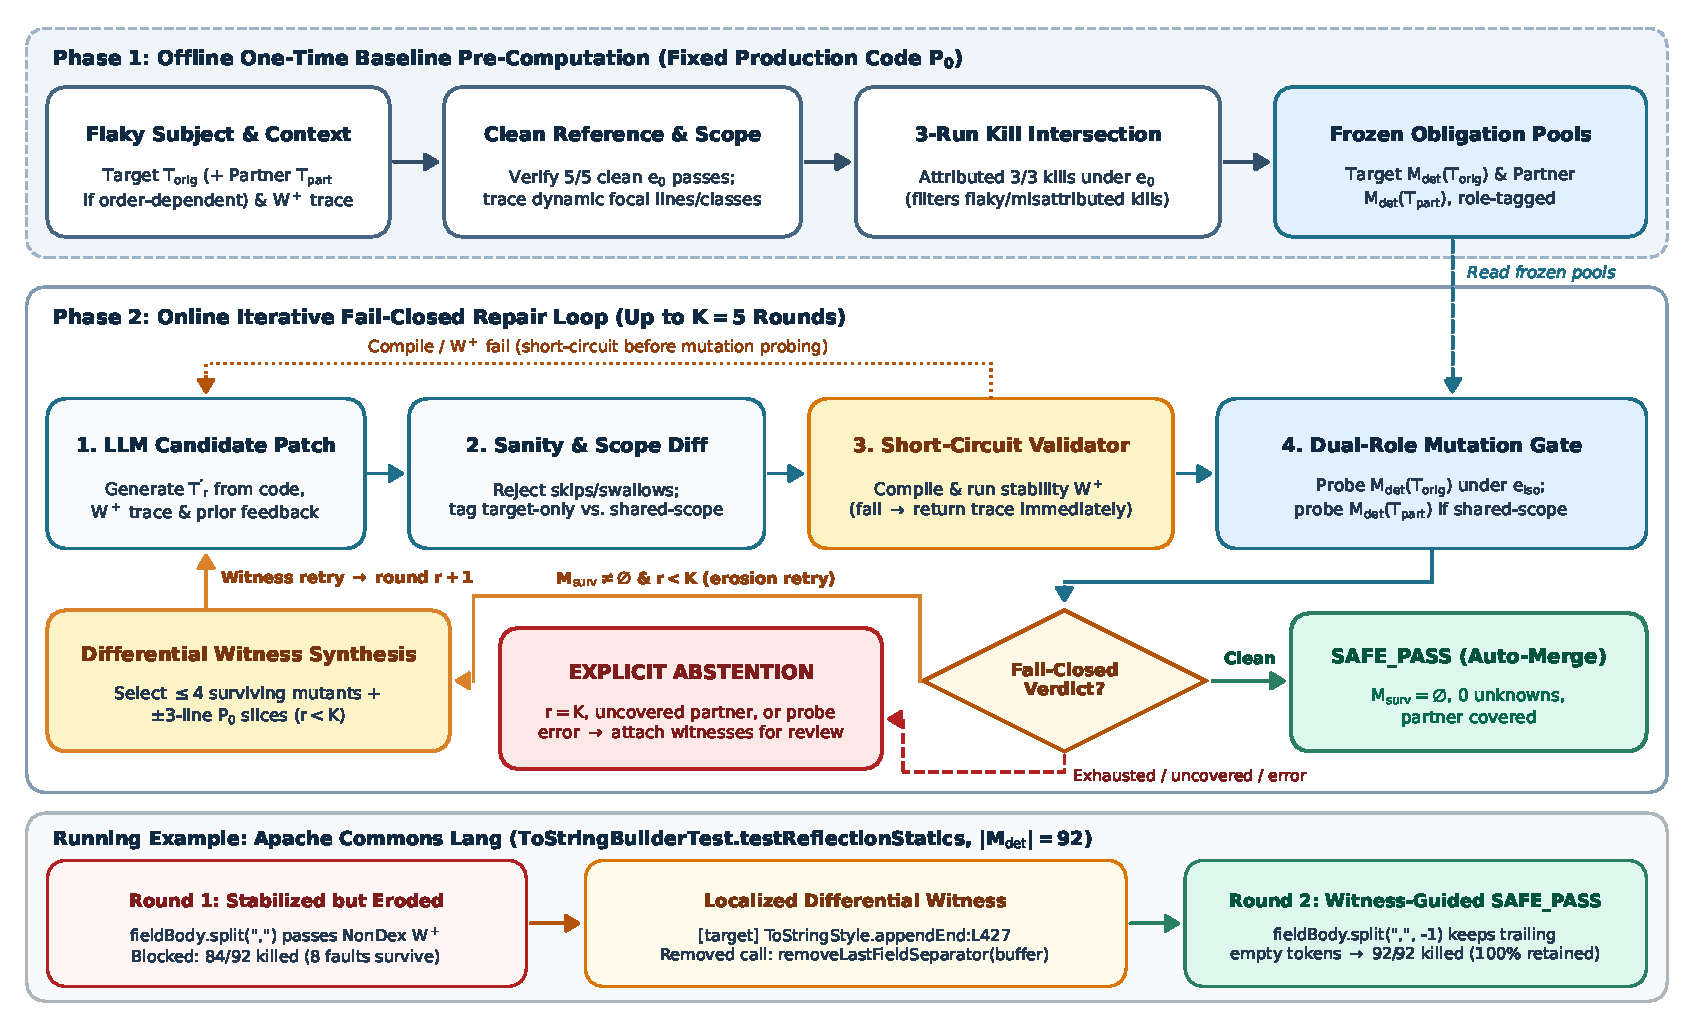
\includegraphics[width=0.93\textwidth]{figures/fig0_muguard_architecture.pdf}
\caption{End-to-end architecture of \textsc{MuGuard-Flake}, showing offline one-time baseline pre-computation, the online fail-closed iterative repair loop, and the two-round \texttt{ToStringBuilderTest} running example.}
\label{fig:architecture}
\end{figure*}

\subsection{Four-Component Fail-Closed Repair Architecture}

\textsc{MuGuard-Flake} pairs offline baseline construction with up to $K = 5$ iterative repair rounds (Algorithm~\ref{alg:muguard}). Given $T_{\text{orig}}$, its $W^+$ failure trace, and surrounding class context (including $T_{\text{part}}$ when order-dependent), each round executes four stages:

\paragraph{Component 1: Single-Test Baseline Pre-Computation.}
Before repair begins, \textsc{MuGuard-Flake} verifies five clean-$e_0$ passes, traces dynamically covered focal scope, and computes the three-run attributed obligation baseline $M_{\text{det}}(T_{\text{orig}})$ from Section~\ref{sec:construct}. Both language backends isolate execution strictly to the target method rather than running whole test classes. For order-dependent tests, partner obligations $M_{\text{det}}(T_{\text{part}})$ are pre-computed independently under the same protocol.

\paragraph{Component 2: Affected-Scope Diff Analysis and Short-Circuit Validator.}
In round $r$, \textsc{MuGuard-Flake} rejects malformed patches (empty bodies, skip markers, or bare exception swallowing) and diffs the target test, partner, and build files, ignoring formatting noise and preserving semantic literals. Edits confined to the target test are tagged \emph{target-only}. Edits touching the partner method, class fields, setup or teardown fixtures, shared helpers, shadowed imports, or build dependencies are tagged \emph{shared-scope} for dual-role gating. The short-circuit validator then compiles candidate $T'_r$ and executes $W^+$. Any compile or stability failure short-circuits immediately and returns diagnostics for the next round without invoking mutation probing.

\paragraph{Component 3: Fail-Closed Dual-Role Conservation Gate.}
Once $T'_r$ passes $W^+$, \textsc{MuGuard-Flake} probes $M_{\text{det}}(T_{\text{orig}})$ under isolated execution $e_{\text{iso}}$ and, for shared-scope order-dependent edits, probes $M_{\text{det}}(T_{\text{part}})$. Two fail-closed invariants govern probing:
\begin{enumerate}[nosep]
    \item \emph{Uncovered-partner closure.} If an order-dependent edit affects shared scope with $|M_{\text{det}}(T_{\text{part}})| = 0$, partner erosion cannot be verified. The gate never accepts the patch, requesting a target-local rewrite on retry or abstaining at round $K$.
    \item \emph{Probe-failure closure.} Any target or partner probe error, timeout, or indeterminate mutant status triggers a retry or abstention rather than silent acceptance or mislabeling as erosion.
\end{enumerate}
Only a clean probe with an empty role-tagged surviving set ($M_{\text{surv}}(T'_r) = \emptyset$) earns a safe pass.

\paragraph{Component 4: Differential Witness Synthesis and Explicit Abstention.}
If $T'_r$ stabilizes with surviving obligations before round $K$, \textsc{MuGuard-Flake} selects up to four role-tagged surviving mutants $m^* \in M_{\text{surv}}(T'_r)$ and synthesizes a localized differential witness:
\begin{equation}
\label{eq:witness}
\begin{aligned}
\omega(m^*) = \big\langle & \text{Role}(m^*),\; \text{Class/File}(m^*),\; \text{Method}(m^*), \\
                          & \text{Line}(m^*),\; \text{OpDesc}(m^*),\; \text{FocalSlice}(P_0, m^*, \pm 3\text{ lines}) \big\rangle.
\end{aligned}
\end{equation}
Following Salva's error-control framing~\cite{salva2026nltestrunner}, if all $K$ rounds end without a clean pass, \textsc{MuGuard-Flake} abstains explicitly rather than merging a degraded test. It records the terminal cause and attaches the surviving-mutant witnesses or failure traces to the pull request, giving human reviewers or hybrid triage assistants concrete production counterexamples to separate valid canonicalization from genuine oracle weakening.

\paragraph{Running Example: Witness-Guided Recovery on \texttt{ToStringBuilderTest}.}
Figure~\ref{fig:architecture} (bottom) traces our Apache Commons Lang running example, \texttt{testReflectionStatics} in \texttt{ToStringBuilderTest} ($|M_{\text{det}}| = 92$). In Round~1, the LLM removes reflection-order flakiness by splitting the serialized field body with single-argument \texttt{split(",")} and sorting the parts. That draft compiles and passes all five \textsc{NonDex} permutations, so single-sided validators accept it immediately. \textsc{MuGuard-Flake}, however, detects eight surviving obligations in \texttt{ToStringStyle} (84/92 killed) and emits the verbatim witness excerpt in Listing~\ref{lst:witness_example}. Pinpointing the removed call to \texttt{removeLastFieldSeparator} reveals that single-argument \texttt{split(",")} drops trailing empty tokens. On Round~2, the model switches to \texttt{split(",", -1)}, restoring 92/92 obligation kills and earning a safe pass.

\begin{lstlisting}[caption={Verbatim differential witness excerpt for Round~1 of \texttt{ToStringBuilderTest} (\texttt{split(",")}, 84/92 killed), exposing the masked trailing-separator fault and guiding Round~2 to \texttt{split(",", -1)} (92/92 killed).},label={lst:witness_example}]
[target] org.apache.commons.lang3.builder.ToStringStyle::appendEnd (L427)
Mutator: VoidMethodCallMutator -- removed call to ToStringStyle::removeLastFieldSeparator
   L425: public void appendEnd(final StringBuffer buffer, final Object object) {
   L426:     if (!this.fieldSeparatorAtEnd) {
>> L427:         removeLastFieldSeparator(buffer);
   L428:     }
   L429:     appendContentEnd(buffer);
\end{lstlisting}

\begin{algorithm}[t]
\caption{\textsc{MuGuard-Flake}: Fail-Closed Mutation-Preserving Flaky Test Repair Loop}
\label{alg:muguard}
\scriptsize
\begin{algorithmic}[1]
\Require Production code $P_0$, flaky test $T_{\text{orig}}$ (and partner $T_{\text{part}}$ if order-dependent), clean config $e_0$, stability family $W^+$, max rounds $K$
\Ensure Terminal gate verdict $d \in \{\texttt{SAFE\_PASS}, \texttt{ABSTAIN\_*}\}$ and verified patch $T^*$ (or $\bot$)
\State Verify $5/5$ clean-$e_0$ passes of $T_{\text{orig}}$; trace focal scope $\mathcal{C}_{\text{focal}}(T_{\text{orig}})$
\State $M_{\text{det}}(T_{\text{orig}}) \gets 3/3$ attributed kills in $\mathcal{C}_{\text{focal}}(T_{\text{orig}})$ under $e_0$
\State If order-dependent, pre-compute standalone $3/3$ attributed partner obligations $M_{\text{det}}(T_{\text{part}})$
\State $\text{feedback} \gets \emptyset$, $T_{\text{prev}} \gets \bot$
\For{$r = 1$ \textbf{to} $K$}
    \State $T'_r \gets \text{LLMRepair}(T_{\text{orig}}, T_{\text{part}}, \text{ContextHeaders}, W^+_{\text{diag}}, T_{\text{prev}}, \text{feedback})$
    \If{$\neg \text{BasicSanity}(T_{\text{orig}}, T'_r)$}
        \State $\text{feedback} \gets \text{SanityErrors}(T'_r)$; $T_{\text{prev}} \gets T'_r$; \textbf{continue}
    \EndIf
    \State $\text{scope} \gets \text{AnalyzeAffectedFileDiff}(T_{\text{orig}}, T_{\text{part}}, T'_r, \text{build})$
    \If{$\neg \text{Compiles}(P_0, T'_r)$}
        \State $\text{feedback} \gets \text{CompileDiagnostics}(P_0, T'_r)$; $T_{\text{prev}} \gets T'_r$; \textbf{continue}
    \EndIf
    \If{$\neg \text{Passes}(P_0, T'_r, W^+)$} \Comment{Short-circuit prior to focal mutation}
        \State $\text{feedback} \gets \text{StabilityTrace}(P_0, T'_r, W^+)$; $T_{\text{prev}} \gets T'_r$; \textbf{continue}
    \EndIf
    \If{order-dependent $\land$ $\text{scope} = \texttt{SHARED\_SCOPE}$ $\land$ $|M_{\text{det}}(T_{\text{part}})| = 0$}
        \State \textbf{if} $r < K$ \textbf{then} $\text{feedback} \gets \text{RequestTargetLocalIsolation}()$; $T_{\text{prev}} \gets T'_r$; \textbf{continue}
        \State \textbf{else} \Return $(\texttt{ABSTAIN\_PARTNER\_UNCOVERED}, \bot)$ \Comment{Fail-closed: never accept}
    \EndIf
    \State $(ok_t, S_t) \gets \text{ProbeFocalMutants}(P_0, T'_r, M_{\text{det}}(T_{\text{orig}}), e_{\text{iso}})$
    \State $(ok_p, S_p) \gets \text{ProbePartnerIfAffected}(P_0, T'_r, T_{\text{part}}, M_{\text{det}}(T_{\text{part}}), \text{scope})$
    \If{$\neg ok_t \lor \neg ok_p$}
        \State \textbf{if} $r < K$ \textbf{then} $\text{feedback} \gets \text{ProbeErrorDiag}()$; $T_{\text{prev}} \gets T'_r$; \textbf{continue}
        \State \textbf{else} \Return $(\texttt{ABSTAIN\_EVAL\_ERROR}, \bot)$ \Comment{Fail-closed on probe failure}
    \EndIf
    \State $M_{\text{surv}} \gets \{(\text{target}, m) \mid m \in S_t\} \cup \{(\text{partner}, m) \mid m \in S_p\}$
    \If{$M_{\text{surv}} = \emptyset$}
        \State \Return $(\texttt{SAFE\_PASS}, T'_r)$
    \ElsIf{$r < K$}
        \State $\Omega \gets \text{ExtractTopWitnesses}(M_{\text{surv}}, w_{\max}=4)$ \Comment{Erosion retry}
        \State $\text{feedback} \gets \text{FormatDifferentialWitness}(\Omega)$; $T_{\text{prev}} \gets T'_r$
    \Else
        \State \Return $(\texttt{ABSTAIN\_EROSION}, \bot)$
    \EndIf
\EndFor
\State \Return $(\texttt{ABSTAIN\_BUILD\_OR\_STABILITY}, \bot)$
\end{algorithmic}
\end{algorithm}

\subsection{Language Backend Implementation}
\label{sec:impl}

Implementing attributed mutation probing and repeated-pollution verification across Java and Python requires strict test isolation to prevent sibling contamination and misattribution.

\paragraph{Java Backend (PIT and JUnit).}
To eliminate sibling-test noise, we snapshot the target test class, mask sibling JUnit~3, 4, and 5 methods before invoking PIT~\cite{coles2016pit} over covered focal classes (default bytecode mutator group), and restore original sources and timestamps afterward. Each mutant carries a lossless eight-field PIT XML signature covering class, method, descriptor, line, mutator, index, block, and description. Kill attribution requires an exact class-and-method match against PIT's killing test, or a class-only match strictly on an isolated single-method class, rejecting substring and superclass matches. Because PIT's XML report does not distinguish \texttt{@Before} setup failures from \texttt{@Test} body failures, held-out repeated-pollution schedules $\langle p_1, p_2, \text{target} \rangle$ use a custom JUnit~4 runner that executes class fixtures once and records per-slot lifecycle verdicts and exception classes. Tests with custom \texttt{@RunWith} runners execute sequentially without phase hooks and never receive stress exemptions.

\paragraph{Python Backend (AST Mutators and Pytest).}
We trace executed same-repository production lines with coverage.py and generate up to 55 deterministic baseline AST mutants across six operator families: comparison negation, boolean swap, negated conditionals, arithmetic swap, constant flips, and \texttt{None} or empty returns. Five unseen AST mutators (augmented assignment, unary operator, dictionary entry, slice bound, and dropped call argument) remain reserved for held-out $M_{\text{ext-op}}$. Offline baseline construction sweeps the full focal pool $M_{\text{focal}}$, and online gating replays only the frozen killed subset $M_{\text{det}}$ under $e_{\text{iso}}$. An instrumented pytest hook enforces exact node and parameter-instance attribution across setup, call, and teardown phases, preventing prefix collisions such as \texttt{test\_loading} versus \texttt{test\_loading\_failure} and failing closed on fixture or partner errors. For held-out repeated-pollution checks, the hook clones the partner test inside a single session, completing the cross-language isolation layer evaluated in Section~\ref{sec:design}.

\section{Experimental Design}
\label{sec:design}

We organize our cross-language study around four research questions, moving from benchmark subjects and blinded audit protocols to repair treatments and project-clustered inference:
\begin{itemize}[nosep]
    \item \textbf{RQ1 (Prevalence and PR Boundaries):} How often does silent oracle erosion occur in historical tools and modern LLMs, and what rejection trade-offs appear on developer pull requests?
    \item \textbf{RQ2 (Mechanisms and Static Blind Spots):} Which edit mechanisms drive erosion, and why do prompt, syntactic, and structural guards fail to block them?
    \item \textbf{RQ3 (Fail-Closed Gating and Witnesses):} How does \textsc{MuGuard-Flake} balance soundness, unseen fault loss, and held-out yield against baselines, and what do witnesses add over scalar counts?
    \item \textbf{RQ4 (Latency, Abstentions, and Subsets):} What uncached probing times and abstention causes arise in practice, and how sensitive is offline detection to smaller mutant subsets?
\end{itemize}

\subsection{Benchmark Cohort, Model Snapshots, and Confirmatory Separation}

We draw an initial cohort of $\BenchInitAttempted$ flaky tests across 70 repositories from two public benchmarks: Java ID and OD-victim tests from \textsc{FlakyDoctor}'s \textsc{IDoFT} suite~\cite{chen2024flakydoctor}, and Python OD-victim and OD-brittle tests from \textsc{iPFlakies}~\cite{wang2022ipflakies}. All builds execute inside hermetic Docker containers under 120\,s timeouts using OpenJDK, Maven, \textsc{NonDex}, and PIT for Java, and isolated virtual environments with pytest and coverage.py for Python. Cohort construction enforced baseline single-probe ceilings of 90\,s in Java and 45\,s in Python, noted as a scope boundary in Section~\ref{sec:threats}.

Applying strict node- and phase-attributed filtering reduced the cohort from $\BenchInitAttempted$ attempted tests to $N = \BenchEligible$ eligible tests across $\BenchProjects$ repositories (Table~\ref{tab:benchmark}). Five tests fell below our three-obligation eligibility floor: four during initial baseline freezing and one after attribution auditing excluded seven inherited JUnit~5 superclass kills. To prevent survivorship bias, we never replace excluded tests. Instead, we report primary metrics on the $\BenchEligible$ eligible tests alongside intent-to-treat (ITT) rates across all $\BenchInitAttempted$ attempted tests.

\begin{table}[t]
\centering
\scriptsize
\setlength{\tabcolsep}{3.6pt}
\caption{Cohort composition and focal obligation profile across $\BenchEligible$ eligible flaky tests in $\BenchProjects$ repositories (five of $\BenchInitAttempted$ attempted tests excluded for fewer than three attributed clean-$e_0$ kills).}
\label{tab:benchmark}
\begin{tabular}{llrrrrrr}
\toprule
Lang. & Subtype & Repos & Elig. & Target $|M_{\text{det}}|$ & Partner $|M_{\text{det}}|$ & $|M_{\text{ext}}|$ (Tests) & Base Probe (s) \\
\midrule
Java & ID (NonDex) & 25 & 61 & 2,089 & 0 (N/A) & 1,777 (61) & 13.02 \\
Java & OD-victim & 11 & 49 & 1,160 & 371 & 1,485 (49) & 7.69 \\
\textit{Java} & \textit{Subtotal} & \textit{35} & \textit{110} & \textit{3,249} & \textit{371} & \textit{3,262 (110)} & \textit{10.21} \\
\midrule
Python & OD-victim & 19 & 60 & 1,154 & 404 & 189 (47) & 11.81 \\
Python & OD-brittle & 16 & 33 & 439 & 262 & 67 (20) & 15.39 \\
\textit{Python} & \textit{Subtotal} & \textit{34} & \textit{93} & \textit{1,593} & \textit{666} & \textit{256 (67)} & \textit{12.29} \\
\midrule
\textbf{Total} & \textbf{Eligible} & \textbf{69} & \textbf{203} & \textbf{4,842} (med.\ 15) & \textbf{1,037} (126/142) & \textbf{3,518} (177) & \textbf{11.69} \\
\bottomrule
\end{tabular}
\par\smallskip\parbox{0.96\textwidth}{\scriptsize\textit{Note:} Base Probe (s) is the median time of one full baseline sweep over the entire focal pool $M_{\text{focal}}$ under $e_0$ (up to 55 Python AST mutants including unkilled ones; OD-brittle replays $\langle T_{\text{set}}, T_{\text{orig}} \rangle$ per mutant). In-loop gating probes only the frozen obligation subset $M_{\text{det}}$ (median 14 in Python; Table~\ref{tab:latency}).}
\end{table}


To prevent harness and guard rules from overfitting to evaluation models, we assign five LLMs across four vendors to three distinct roles. All five models were invoked via official vendor APIs during our November 2026 campaign at temperature 0.0, a 6,144-token output cap, and a 16k reasoning-token limit. Our exact API identifiers are \texttt{deepseek-flash} and \texttt{deepseek-v4-pro} from DeepSeek, \texttt{qwen3.7-plus} from Alibaba Cloud, \texttt{kimi-k2.5} from Moonshot AI, and \texttt{glm-5} from Zhipu AI, with complete prompt--response caches archived in the replication package. DeepSeek Flash and DeepSeek V4 Pro served as \emph{exploratory} multi-round backbones during guard development, and Alibaba Qwen 3.7 Plus acts as our pre-specified \emph{confirmatory} multi-round backbone. Single-pass runs on Kimi K2.5 and GLM-5 test cross-family generalization. Before confirmatory evaluation, we locked attribution, bytecode restoration, phase isolation, and guard rules under a 19-test regression suite, re-running downstream rounds end to end whenever a revision altered an earlier decision.

\subsection{Historical Artifacts, Pull Requests, Blinded Cross-Audit, and Strategies}

\paragraph{Historical Repair Artifacts.}
We restrict historical auditing to official upstream passing entries: patches marked passing in \textsc{FlakyDoctor}'s GPT-4 and Magicoder logs and partner-matched rows in \textsc{iPFlakies}'s official patch log. Unlogged archive files and three partner-mismatched Python rows are excluded. Each official patch is applied verbatim without manual edits and evaluated through the same attribution harness.

\paragraph{Developer Pull Requests and Blinded Dual-Auditor Reliability Protocol.}
To measure false rejections on valid human fixes and subtle weakenings missed by default mutators, we collect $\PRTotalInstances$ Java instances across $\PRDistinctURLs$ \textsc{IDoFT} pull requests. Test-file application is strictly atomic across one shared repository tree, and stabilized test-only order-dependent pull requests pass through the full dual-role gate.

All three semantic-adjudication tasks follow one two-stage blinded reliability protocol spanning all 53 cleanly applied pull requests (43 $W^+$-passing test-only), the 55 active diff-matched patches from our 60-patch stratified draw (five earlier pre-revision snapshots were replaced during end-to-end re-execution), and all 111 unique held-out $M_{\text{ext}}$-loss patches. In Stage~1, the first author classified every patch from original-versus-patched diffs under a frozen rubric decoupled from gate verdicts.

In Stage~2, an independent automated auditor---OpenAI Codex CLI v0.153.4 (\texttt{gpt-6-astra}, medium reasoning effort, November 2026)---re-adjudicated every patch inside a physically isolated read-only workspace containing solely code diffs and mutant lists. Stage~2 remained strictly blinded to strategy names, model identities, gate verdicts, PR merge status, and Stage-1 labels; using an independent U.S.-provider auditor on patches from four Chinese-provider repair models also avoids same-family self-preference bias. We quantify pre-arbitration agreement via unweighted Cohen's $\kappa$~\cite{cohen1960kappa} and resolve all 35 primary-decision disagreements---3 PR legitimacy boundaries, 7 erosion-mechanism labels, and 25 held-out $W/S/L$ labels---via third-pass evidence-grounded arbitration archived in our replication package:
\begin{itemize}[nosep]
    \item \emph{Pull-request audit.} Five-class agreement across all 53 evaluated PRs reaches 84.9\% ($\kappa = 0.74$, 8 label differences). Across the 43 $W^+$-passing test-only fixes, legitimate versus non-legitimate agreement reaches 93.0\% ($\kappa = 0.63$), leaving only 3 legitimacy-boundary cases for arbitration (including the Apache Avro shift in Section~\ref{sec:rq1}; the other 5 differences split two legitimate subtypes).
    \item \emph{Stratified erosion audit.} Across the 55 active diffs, seven-class mechanism agreement reaches 87.3\% ($\kappa = 0.83$, 7 arbitrated cases), and non-legitimate erosion versus legitimate relaxation reaches 98.2\% ($\kappa = 0.79$). Splitting non-legitimate edits further into genuine degradation versus responsibility shift yields three-way $\kappa = 0.24$, as 27 of 28 fine-grained differences divide degradation from shift on fixture-narrowing edits without questioning non-legitimacy.
    \item \emph{Held-out $M_{\text{ext}}$-loss audit.} Three-class $W/S/L$ agreement across all 111 loss patches reaches 77.5\% ($\kappa = 0.66$, 25 arbitrated cases). Blinded Stage-2 labels reproduce identical \textsc{MuGuard-Flake} $W/S/L$ counts on DeepSeek V4 Pro and Qwen 3.7 Plus and widen its advantage over baselines on weakening and shift losses.
\end{itemize}
Section~\ref{sec:threats} records the construct boundary of using an automated Stage-2 auditor rather than a second human annotator.

\paragraph{Six Controlled Repair Strategies ($K=5$, Temperature 0.0).}
Holding localization headers, partner code, stability traces, output schema, and retry budget identical, we compare six strategies:
\begin{enumerate}[nosep]
    \item \emph{Unconstrained.} Accepts the first compiled, $W^+$-passing candidate passing basic non-empty, no-skip, and exception-swallowing sanity checks.
    \item \emph{Prompt Guard.} Adds explicit contract-preservation instructions prohibiting assertion deletion, projection relaxation, substring fallbacks, and state clobbering.
    \item \emph{Syntactic Guard.} Enforces assertion-count preservation and blocks trivial tautologies, skip annotations, and exception swallowing prior to compilation.
    \item \emph{Structural Guard.} Extends static checking with assertion-level correspondence rules built from exploratory syntactic bypasses and evaluated out-of-sample on Qwen 3.7 Plus, Kimi K2.5, and GLM-5. It flags projection downgrades, dual-call tautologies, missing focal calls, and post-action state resets.
    \item \emph{Scalar Gate.} Executes the exact fail-closed $W^+ \times M_{\text{det}}$ mutation gate of \textsc{MuGuard-Flake}, returning only the surviving count $k/M$ on erosion retries without code locations.
    \item \emph{MuGuard-Flake.} Pairs the fail-closed mutation gate with localized surviving-mutant witnesses (Algorithm~\ref{alg:muguard}).
\end{enumerate}

\subsection{Prefix-Forked Witness Experiment and Clustered Statistical Inference}

\paragraph{Prefix-Forked Witness Experiment.}
To isolate whether accurate fault localization drives recovery beyond extra retries or longer prompts, every multi-round trajectory triggering its first erosion retry before round~5 enters a paired fork pool. This pool spans $n = \ForkTotal$ forks across $\ForkTests$ tests in $\ForkProjects$ repositories; two round-5 triggers lack remaining budget and stay in full-cohort totals. From each identical pre-fork state, four arms share the remaining budget. \emph{Gate-Only} abstains immediately at 0\% recovery by definition, and \emph{Scalar Ratio} returns only $k/M$. \emph{Misleading Witness} keeps the witness template and mutant count identical using already-killed mutants, completing $\ForkTotalATwo$ forks after 12 API token-cap omissions. \emph{True Witness} supplies the localized surviving-mutant package. True Witness versus Scalar Ratio across all $\ForkTotal$ forks serves as our pre-registered primary mechanism test.

\paragraph{Project-Clustered Paired Inference.}
Because flaky tests cluster within repositories, treating tests as independent understates variance. Every paired comparison therefore estimates test-weighted risk differences in percentage points alongside 95\% whole-repository cluster bootstrap confidence intervals over 20,000 resamples. We treat a five-point lift as the minimum practical gain and report equal-repository averages as a sensitivity check. Hypothesis tests use paired project-level Rademacher sign-flip permutations, enumerating exact assignments whenever non-zero-difference repositories do not exceed 16. Holm--Bonferroni adjustment at the 5\% significance level controls familywise error across three pre-registered families: operational soundness against non-mutation baselines, fixed-cohort held-out yield, and witness recovery. Section~\ref{sec:results} presents our empirical findings.

\section{Empirical Results}
\label{sec:results}

We evaluate oracle erosion across $N = \BenchEligible$ flaky tests in $\BenchProjects$ repositories and 1,243 unique held-out candidate patches. We first quantify erosion prevalence and developer pull-request boundaries (RQ1), then diagnose why static guards miss behavioral shifts (RQ2) before assessing fail-closed mutation gating, asymmetric CI cost, and runtime overhead (RQ3--RQ4).

\subsection{RQ1: Prevalence of Silent Oracle Erosion and Pull-Request Boundaries}
\label{sec:rq1}

\paragraph{Historical Repair Artifacts.}
Silent oracle erosion is already pervasive in published flaky-test repair artifacts (Table~\ref{tab:b1_sota}). Among official upstream passing entries from \textsc{FlakyDoctor} GPT-4, nearly half compile verbatim and pass stability reruns, yet \BOneGptLeakPct{} of those stabilized patches silently drop baseline fault obligations. That erosion lowers operational sound-fix yield by 12 percentage points. By contrast, none of the four matched and stabilized \textsc{FlakyDoctor} Magicoder patches erode obligations, though four patches are too few to support model-level conclusions.

Python suite-search patching exhibits nearly the same erosion rate as LLM-based Java repair. Among partner-matched official \textsc{iPFlakies} entries, \BOneIpfLeakPct{} of stabilized fixes lose baseline obligations, opening a 13-point gap between apparent stabilization and sound repair. Silent erosion is therefore not unique to language models. Whenever a repair pipeline rewards green execution without checking fault detection, both search-based splicers and generative agents gravitate toward edits that silence intermittent failures at the cost of weaker assertions or shallower fixture states.

\begin{table}[t]
\centering
\footnotesize
\setlength{\tabcolsep}{3.0pt}
\caption{Audit of official upstream passing patches from \textsc{FlakyDoctor} and partner-matched \textsc{iPFlakies} artifacts under unified attribution. Bold marks silent oracle erosion among $W^+$-passing fixes.}
\label{tab:b1_sota}
\begin{tabular}{lrrrrrrr}
\toprule
Historical Artifact Cohort & Avail. & Mism. & Comp. & Pass@$W^+$ & Eroded & Leak ($W^+$) & SoundFix \\
\midrule
FlakyDoctor GPT-4 (official pass) & 75 & 20 & 38 & 33 (44.00\%) & \textbf{9} & \textbf{27.27\%} & 24 (32.00\%) \\
FlakyDoctor Magicoder (official pass) & 13 & 6 & 4 & 4 (30.77\%) & \textbf{0} & \textbf{0.00\%} & 4 (30.77\%) \\
iPFlakies (partner-matched) & 77 & 0 & 60 & 42 (54.55\%) & \textbf{10} & \textbf{23.81\%} & 32 (41.56\%) \\
\bottomrule
\end{tabular}
\end{table}


\paragraph{Modern LLM Backbones Across Five Models.}
Unconstrained LLM repair loops show consistent erosion rates across all five models from four vendors (Figure~\ref{fig:inflation_gap}, Table~\ref{tab:k5_operational}, and Table~\ref{tab:crossfamily_r1}). Under multi-round validation, API reasoning-token limits truncated one eligible test on DeepSeek Flash and 15 on DeepSeek V4 Pro, whereas confirmatory Qwen 3.7 Plus completed the full cohort. Silent erosion affects roughly one-fifth to one-quarter of stabilized patches on every backbone. Combined with the explicit \emph{Unver.} column in Table~\ref{tab:k5_operational}---unverified shared-scope partner edits plus one indeterminate target timeout on DeepSeek Flash and DeepSeek V4 Pro Unconstrained---these losses open a Proxy Inflation Gap of 24 to 26 percentage points across backbones.

Single-pass screening across two additional model families confirms that this gap generalizes beyond DeepSeek and Qwen. Without multi-round retries, unconstrained Kimi K2.5 leaks 26.8\% eroded patches among its stabilized outputs, and GLM-5 leaks 25.6\%. Across both reasoning and non-reasoning models, green stability checks overstate sound repair rates by roughly a quarter. This uniformity points to a structural incentive flaw rather than a quirk of any single model family. Because stabilization checks penalize every flaky failure immediately but never penalize a missing assertion check, stronger models simply become more adept at finding permissive edits that turn tests green quickly.

\begin{figure*}[t]
\centering
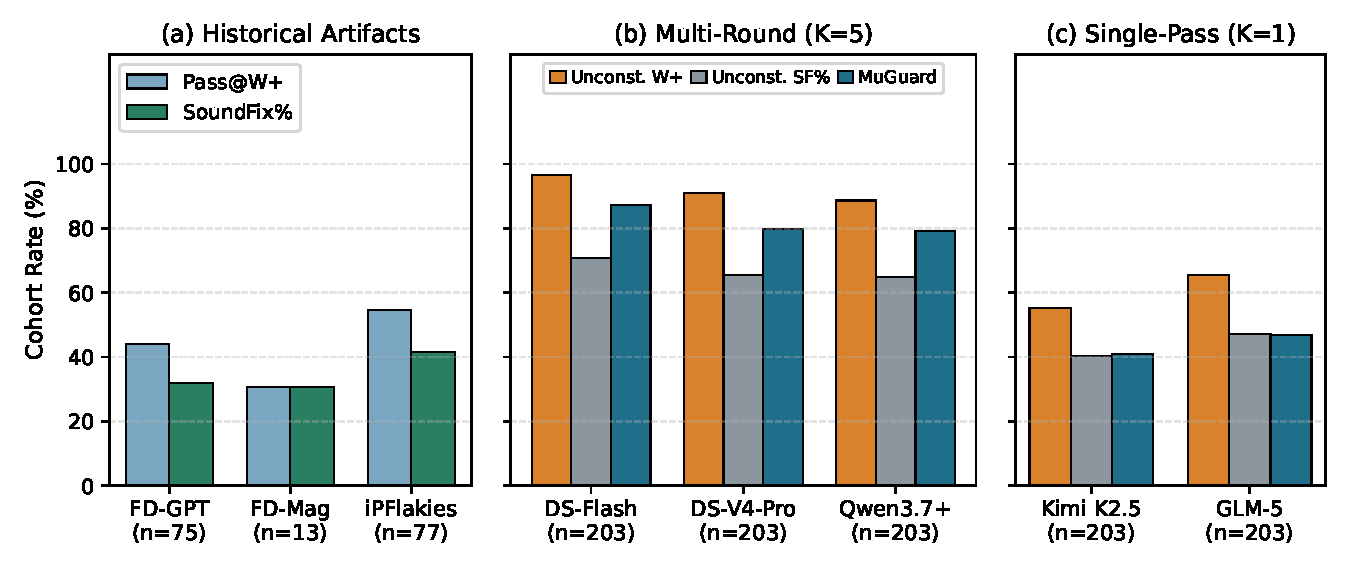
\includegraphics[width=0.98\textwidth]{figures/fig1_inflation_gap_models.pdf}
\caption{Apparent stabilization pass rate versus operational sound-fix rate across historical artifacts, multi-round LLM repair, and single-pass cross-family screening.}
\label{fig:inflation_gap}
\end{figure*}

\paragraph{Developer Pull Requests and the False-Rejection Boundary.}
Auditing real human fixes exposes both the false-rejection cost and the incomplete recall of strict mutation gating (Table~\ref{tab:pr_adjudication}). Across $\PRTotalInstances$ Java instances from $\PRDistinctURLs$ GitHub pull requests, 45 test-only fixes apply cleanly and 43 pass stability reruns, including all 24 order-dependent cases. Focusing on the 16 merged fixes that stabilize, Syntactic Guard rejects one, Structural Guard rejects three, and \textsc{MuGuard-Flake} rejects two. Diff adjudication---corroborated at 93.0\% agreement ($\kappa = 0.63$) by our blinded cross-audit---reveals opposite semantics for those two rejections: one Fastjson pull request legitimately enables deterministic map-key sorting, and a Nacos pull request replaces exact JSON equality with partial substring checks that genuinely weaken the oracle.

Across all $\PRLegitTotal$ verified legitimate test-only repairs, strict \textsc{MuGuard-Flake} gating rejects eight fixes, a \PRLegitFalseRejMuGuardPct{} false-rejection rate (or 22.5\% if the single Apache Avro responsibility-shift fix is included). Those eight false rejections stem from two concrete patterns: three Fastjson canonicalization fixes that bypass unsorted serialization branches, and five Visualee fixtures whose \texttt{@Before} singleton cleanup lowers PIT kill counts without altering any assertion. Conversely, manual review surfaced three genuine weakening pull requests among stabilized fixes. \textsc{MuGuard-Flake} and Structural Guard both catch the Nacos substring downgrade, and two subtle merged weakenings in Commons Collections and Apollo retain all default PIT kills and escape every gate.

These pull-request cases sharpen how strict mutation gating should be interpreted in practice. A strict gate does not separate legitimate fixes from broken ones with perfect precision, because valid canonicalization or fixture cleanup can legitimately change which production branches a test traverses. At the same time, default bytecode operators cannot expose every subtle relational weakening, such as dropping a cross-entry key-to-value bijection. Strict mutation gating therefore operates as an auditable safety filter with concrete false-rejection and false-negative boundaries rather than an omniscient oracle.

\begin{table}[t]
\centering
\scriptsize
\setlength{\tabcolsep}{2.4pt}
\caption{Gate rejection and weakening-detection rates across $W^+$-passing test-only developer pull requests comparing static, coverage, cross-vendor LLM-judge, strict \textsc{MuGuard-Flake}, and witness-augmented hybrid triage.}
\label{tab:pr_adjudication}
\begin{tabular}{llrrrrr}
\toprule
PR Cohort & $n$ & Structural & Coverage$^{\dagger}$ & LLM-Judge & MuGuard & MuGuard+Triage \\
\midrule
Merged Test-Only ($W^+$) & 16 & 3/16 (18.75\%) & 1/13 (7.7\%) & 2/16 (12.5\%) & 2/16 (12.50\%) & \textbf{1/16 (6.3\%)} \\
Legitimate Fixes (Primary) & 39 & 4/39 (10.3\%) & 2/32 (6.3\%) & 3/39 (7.7\%) & 8/39 (20.5\%) & \textbf{0/39 (0.0\%)} \\
Legit.\ + Shift (Sens.) & 40 & 4/40 (10.0\%) & 2/32 (6.3\%) & 3/40 (7.5\%) & 9/40 (22.5\%) & \textbf{0/40 (0.0\%)} \\
\midrule
Genuine Weakening (TP) & 3 & 1/3 (33.3\%) & 0/2 (0.0\%) & \textbf{3/3 (100\%)} & 1/3 (33.3\%) & 1/3 (33.3\%) \\
\bottomrule
\end{tabular}
\par\smallskip\parbox{0.97\textwidth}{\scriptsize\textit{Note:} Syntactic Guard rejects 1/39 (2.6\%) legitimate PRs and catches 0/3 weakenings. $^{\dagger}$JaCoCo executed on 34/43 Java PRs (9 blocked by upstream Maven \texttt{argLine} conflicts). LLM-Judge uses cross-vendor Qwen 3.7 Plus (Zhipu GLM-5 yields 2/39 = 5.1\% false rejections and 3/3 weakenings). Under our stricter 10-session blinded Codex ensemble rubric (Fleiss' $\kappa=1.00$), which classifies Visualee global singleton wipes as responsibility shifts, strict \textsc{MuGuard-Flake} rejects only 1/29 (3.4\%) strictly contract-preserving PRs.}
\end{table}


\medskip
\noindent\fbox{\parbox{0.97\textwidth}{\textbf{Summary for RQ1:} Silent oracle erosion affects roughly one in five to one in four stabilization-passing patches across historical tools and five modern LLM families. On audited developer pull requests, strict mutation gating incurs a \PRLegitFalseRejMuGuardPct{} false-rejection rate on legitimate fixes and misses two of three subtle weakening patches outside default mutators.}}
\medskip

Given how consistently silent erosion emerges across tools and models, RQ2 examines which concrete edit patterns erode obligations and why static guards fail to intercept them.

\subsection{RQ2: Behavioral Erosion Mechanisms and Static-Guard Blind Spots}
\label{sec:rq2}

Static checks fail to curb silent erosion and can even harm repair yield (Tables~\ref{tab:k5_operational} and~\ref{tab:crossfamily_r1}). Contract-preservation prompts and syntactic assertion-count checks do not consistently reduce leaked erosion relative to unconstrained repair, slightly increasing leakage on both DeepSeek models and reducing it by barely one percentage point on Qwen. Even the strengthened Structural Guard still leaks \FlashBThreePlusLeakPct{} to \ProBThreePlusLeakPct{} eroded patches across the three multi-round models. Worse, it lowers operational sound-fix yield below Syntactic Guard on every backbone, including a 3.9-point drop on confirmatory Qwen 3.7 Plus.

Two competing forces explain why stricter static heuristics underperform. Static pattern rules block legitimate structural rewrites when developers or models reorganize assertions, as reflected in Structural Guard's 18.8\% rejection rate on merged test-only pull requests. At the same time, rejecting obvious syntactic shortcuts nudges models toward subtler behavioral edits that keep every assertion statement intact while changing what production code executes. Rather than solving erosion, aggressive syntax rules trade transparent assertion edits for harder-to-spot behavioral shifts.

\begin{table}[t]
\centering
\scriptsize
\setlength{\tabcolsep}{2.7pt}
\caption{Edit-mechanism distribution and cross-paradigm bypass counts across $\TaxUniquePatches$ unique $W^+$-passing eroded patches in $\TaxDistinctProjects$ repositories, paired with the 60-patch active stratified audit.}
\label{tab:taxonomy}
\begin{tabular}{lrrrrr}
\toprule
Patch Edit Mechanism & Auto Prim. & Bypass Struct. & Bypass Judge & Bypass Cov.$^{\dagger}$ & Audit ($N=60$) \\
\midrule
Predicate Projection or Relaxation & 10 & 5 & 3 & 8/10 & 2 \\
State Reset or Post-Act Clobber & 26 & 7 & 26 & 26/26 & 4 \\
Control-Flow or Exception Shift & 0 & 0 & 0 & 0/0 & 2 \\
Focal Call Alteration or Bypass & 52 & 48 & 39 & 17/52 & 9 \\
Partner or Shared-Scope Side-Effect & 53 & 43 & 49 & 40/53 & 4 \\
Delimiter or Format Normalization & 112 & 86 & 64 & 106/112 & 14 \\
Precondition or Singleton Setup Shift & 120 & 119 & 111 & 63/120 & 25 \\
Unclassified Residual & 27 & 27 & 20 & 8/26 & 0 \\
\midrule
\textbf{Total Eroded Patches (Bypass\%)} & \textbf{400} & \textbf{335 (83.8\%)} & \textbf{312 (78.0\%)} & \textbf{268/399 (67.2\%)} & \textbf{60} \\
\bottomrule
\end{tabular}
\par\smallskip\parbox{0.97\textwidth}{\scriptsize\textit{Note:} Syntactic Guard is bypassed by 396/400 (99.0\%) patches; \textsc{MuGuard-Flake} intercepts all 400/400 (0\% bypass) by definition. $^{\dagger}$Dynamic focal line Coverage Gate (JaCoCo + \texttt{coverage.py}) evaluated on 399/400 patches with clean baseline coverage (1 Java patch had an upstream Maven \texttt{argLine} conflict).}
\end{table}


Over four-fifths of unique eroded patches across \TaxDistinctProjects{} repositories bypass Structural Guard, and nearly all bypass Syntactic Guard (Table~\ref{tab:taxonomy}). Our stratified manual audit confirms that nearly three-quarters represent genuine fault-detection weakening, one-fifth shift test responsibility, and only four patches reflect legitimate canonicalization, matching automated mechanism labels on 92.7\% of active patches. Blinded cross-auditing independently confirms strong mechanism agreement ($\kappa = 0.83$) and near-unanimous non-legitimacy agreement ($\kappa = 0.79$). Across mutator families, eroded patches blind tests primarily to branch-condition faults, followed by value-return and side-effect call faults.

Four behavioral blind spots account for most static-guard bypasses:
\begin{enumerate}[nosep]
    \item \emph{Precondition and singleton setup shifts} (119 of 120 patches bypass Structural Guard). Minimal fixture setups preserve every assertion while skipping deeper production branches. In Python \texttt{NestedDictionary::test\_del} (Listing~\ref{lst:case_e3}), Structural Guard accepts the same single-key setup produced by \textsc{iPFlakies}, leaving the dictionary empty after deletion until \textsc{MuGuard-Flake}'s witness restores a sibling key.
    \item \emph{Delimiter and format normalizations} (86 of 112 patches bypass Structural Guard). In our Java running example \texttt{ToStringBuilderTest.testReflectionStatics} (Figure~\ref{fig:architecture}, Listings~\ref{lst:witness_example} and~\ref{lst:case_e1}), Structural Guard accepts single-argument \texttt{split(",")}, which silently strips trailing empty tokens and misses eight faults in \texttt{ToStringStyle} until the witness induces \texttt{split(",", -1)}.
    \item \emph{Partner-test and shared-fixture edits} (43 of 53 patches bypass Structural Guard). Editing a partner test or shared setup block leaves target assertions untouched while silently dropping partner obligations.
    \item \emph{Focal call alteration or bypass} (48 of 52 patches bypass Structural Guard). In Java \texttt{HttpRequestTest} (Listing~\ref{lst:case_e4}), substituting an anonymous factory stub bypasses \texttt{ConnectionFactory.DEFAULT} while preserving every assertion statement.
\end{enumerate}

A common thread links all four blind spots. None of these edits looks suspicious under local syntactic inspection of the assertion block itself: every assertion call remains present, non-trivial, and properly typed. Instead, the fault-detection loss happens upstream in the fixture, the input parser, the shared helper, or the mocked collaborator. Catching such regressions requires executing the repaired test against mutated production behavior rather than pattern-matching its syntax tree.

\begin{lstlisting}[language=Python,caption={Precondition shift in \texttt{NestedDictionary::test\_del}, where a single-key setup accepted by \textsc{iPFlakies} and Structural Guard skips a nested lookup path until witness feedback restores a sibling key.},label={lst:case_e3}]
# Official iPFlakies and Structural Guard Accepted Patch (Retention = 4/5):
def test_del(x):
    x[123] = 'abc'        # Dict becomes empty after del -> skips _look_deeper:L41
    del x[123]
    with raises(KeyError): assert x[123]

# MuGuard-Flake Witness (easy_dict._look_deeper:L41) -> Round-2 Safe Pass (5/5):
def test_del(x):
    x[123] = 'abc'; x['def'] = 456  # Preserves non-empty sibling lookup path
    del x[123]
    with raises(KeyError): assert x[123]
\end{lstlisting}

\begin{lstlisting}[language=Java,caption={Format normalization in \texttt{ToStringBuilderTest.testReflectionStatics}, where single-argument \texttt{split(",")} drops trailing-token checks under Structural Guard until witness feedback restores \texttt{split(",", -1)}.},label={lst:case_e1}]
// Structural Guard Accepted Patch (Passes NonDex; Retention = 84/92):
final List<String> fields = new ArrayList<>(Arrays.asList(fieldBody.split(",")));

// MuGuard-Flake Witness (ToStringStyle.appendEnd:L427) -> Round-2 Safe Pass (92/92):
final List<String> fields = new ArrayList<>(Arrays.asList(fieldBody.split(",", -1)));
\end{lstlisting}

\begin{lstlisting}[language=Java,caption={Focal call bypass in \texttt{HttpRequestTest}, where an anonymous factory stub bypasses \texttt{ConnectionFactory.DEFAULT} under Structural Guard until witness feedback restores the default factory.},label={lst:case_e4}]
// Structural Guard Accepted Patch (Assertions untouched; Retention = 21/22):
HttpRequest.setConnectionFactory(new ConnectionFactory() { ... });

// MuGuard-Flake Witness (ConnectionFactory$1.create:L389) -> Round-2 Safe Pass (22/22):
HttpRequest.setConnectionFactory(ConnectionFactory.DEFAULT);
\end{lstlisting}

\medskip
\noindent\fbox{\parbox{0.97\textwidth}{\textbf{Summary for RQ2:} Over four-fifths of unique eroded patches bypass an enhanced static structural guard through behavioral setup shifts, delimiter normalizations, shared-scope edits, and focal call bypasses. Stratified auditing confirms that nearly three-quarters represent genuine fault-detection degradation.}}
\medskip

Because static rules cannot intercept these behavioral shifts, RQ3 evaluates whether executable mutation gating and surviving-mutant witnesses close the gap.

\subsection{RQ3: Fail-Closed Gating Trade-Off, External Validation, and Witness Recovery}
\label{sec:rq3}

\paragraph{Operational Sound-Fix Gains Across Five Models.}
Under fail-closed mutation gating, \textsc{MuGuard-Flake} eliminates leaked in-loop erosion across all multi-round models and lifts operational sound-fix yield far above our 5-point practical threshold (Tables~\ref{tab:k5_operational} and~\ref{tab:stat_tests}). On confirmatory Qwen 3.7 Plus, it reaches \QwenOursSoundPct{} operational sound-fix yield, beating unconstrained and static baselines by 12 to 16 percentage points. Exploratory DeepSeek Flash and DeepSeek V4 Pro show a similar 15- to 18-point advantage over every non-mutation baseline. Every primary test-weighted gain survives whole-repository clustering and Holm--Bonferroni correction, with positive equal-repository point estimates throughout.

Two mechanisms combine to produce these large operational gains. First, the gate immediately blocks every stabilized candidate that silently drops baseline obligations or alters uncovered shared scope, removing the erosion and unverified leakage that drag down unconstrained and static-guarded loops. Second, rather than discarding those blocked candidates, witness-guided retries convert most intercepted erosions into clean, obligation-preserving repairs within the remaining iteration budget. This pairing explains why \textsc{MuGuard-Flake} lifts sound-fix yield consistently across models with different reasoning styles and base repair capacities.

\begin{table}[t]
\centering
\scriptsize
\setlength{\tabcolsep}{2.8pt}
\caption{Multi-round ($K=5$) operational repair outcomes across exploratory DeepSeek and confirmatory Qwen backbones. On every row, $\text{SoundFix} = \text{Pass@}W^+ - \text{Leaked} - \text{Unver.}$}
\label{tab:k5_operational}
\begin{tabular}{llrrrrrr}
\toprule
Model ($n_{\text{elig}}$) & Strategy & Pass@$W^+$ & Leaked ($W^+$) & Unver. & SoundFix\% [95\% CI] & ITT\% & Joint Ret. \\
\midrule
DS-Flash (202) & Unconstrained & 196 (97.03\%) & 39 (19.90\%) & 13 & 71.29\% [59.7, 82.1] & 69.23\% & 0.9659 \\
 & Prompt Guard & 197 (97.52\%) & 40 (20.30\%) & 13 & 71.29\% [61.8, 81.1] & 69.23\% & 0.9677 \\
 & Syntactic Guard & 198 (98.02\%) & 41 (20.71\%) & 13 & 71.29\% [61.8, 81.1] & 69.23\% & 0.9674 \\
 & Structural Guard & 195 (96.53\%) & 41 (21.03\%) & 13 & 69.80\% [59.6, 80.1] & 67.79\% & 0.9760 \\
 & Scalar Gate & 162 (80.20\%) & 0 (0.00\%) & 0 & 80.20\% [69.0, 90.7] & 77.88\% & 1.0000 \\
 & \textbf{MuGuard-Flake} & 177 (87.62\%) & \textbf{0 (0.00\%)} & 0 & \textbf{87.62\% [78.7, 95.2]} & 85.10\% & 1.0000 \\
\midrule
DS-V4-Pro (188) & Unconstrained & 177 (94.15\%) & 42 (23.73\%) & 4 & 69.68\% [59.6, 80.2] & 62.98\% & 0.9623 \\
 & Prompt Guard & 174 (92.55\%) & 43 (24.71\%) & 5 & 67.02\% [57.1, 77.1] & 60.58\% & 0.9583 \\
 & Syntactic Guard & 181 (96.28\%) & 46 (25.41\%) & 5 & 69.15\% [60.0, 78.8] & 62.50\% & 0.9589 \\
 & Structural Guard & 182 (96.81\%) & 49 (26.92\%) & 5 & 68.09\% [58.6, 78.1] & 61.54\% & 0.9533 \\
 & Scalar Gate & 147 (78.19\%) & 0 (0.00\%) & 0 & 78.19\% [65.8, 89.4] & 70.67\% & 1.0000 \\
 & \textbf{MuGuard-Flake} & 160 (85.11\%) & \textbf{0 (0.00\%)} & 0 & \textbf{85.11\% [73.2, 94.2]} & 76.92\% & 1.0000 \\
\midrule
Qwen3.7+ (203) & Unconstrained & 180 (88.67\%) & 37 (20.56\%) & 11 & 65.02\% [53.2, 76.7] & 63.46\% & 0.9603 \\
 & Prompt Guard & 180 (88.67\%) & 35 (19.44\%) & 8 & 67.49\% [56.9, 78.6] & 65.87\% & 0.9624 \\
 & Syntactic Guard & 180 (88.67\%) & 36 (20.00\%) & 8 & 67.00\% [55.6, 78.9] & 65.38\% & 0.9620 \\
 & Structural Guard & 175 (86.21\%) & 39 (22.29\%) & 8 & 63.05\% [50.9, 75.8] & 61.54\% & 0.9573 \\
 & Scalar Gate & 153 (75.37\%) & 0 (0.00\%) & 0 & 75.37\% [64.7, 85.6] & 73.56\% & 1.0000 \\
 & \textbf{MuGuard-Flake} & 161 (79.31\%) & \textbf{0 (0.00\%)} & 0 & \textbf{79.31\% [68.3, 89.2]} & 77.40\% & 1.0000 \\
\bottomrule
\end{tabular}
\par\smallskip\parbox{0.97\textwidth}{\scriptsize\textit{Note:} $n_{\text{elig}}$ omits runs hitting the 16k reasoning-token API cap (1 on DS-Flash, 15 on DS-V4-Pro; Qwen3.7+ completed all 203); ITT\% divides eligible sound fixes by all $\BenchInitAttempted$ attempted tests. Unver.\ counts $W^+$-passing candidates withheld from SoundFix under fail-closed conservation: unverified shared-scope edits where $|M_{\text{det}}(T_{\text{part}})|=0$ (12 on DS-Flash, 3--5 on DS-V4-Pro, 8--11 on Qwen3.7+) plus 1 indeterminate target probe timeout on DS-Flash (all four non-mutation strategies) and DS-V4-Pro Unconstrained.}
\end{table}


Single-pass screening on Kimi K2.5 and GLM-5 confirms that the admission gate transfers across model families even without retries (Table~\ref{tab:crossfamily_r1}). On both models, \textsc{MuGuard-Flake} blocks every eroded first-round patch, intercepting 30 on Kimi K2.5 and 34 on GLM-5 without sacrificing single-pass sound-fix yield. It edges past Structural Guard by two percentage points on each model. These single-pass results show that mutation gating protects build quality immediately on round one, before iterative witness recovery even begins.

\paragraph{External Validation: Conditional Safety vs.\ Unconditional Yield Trade-Off.}
External validation across all 1,243 candidate patches on disjoint schedules and unseen fault obligations ($|E| = \BenchMExtSamples$) exposes a sharp risk--coverage trade-off (Table~\ref{tab:k5_heldout}). Among accepted patches, \textsc{MuGuard-Flake} cuts conditional unseen-obligation loss substantially on every model: by \FlashRelRedVsBZeroPct{} to \QwenRelRedVsBZeroPct{} versus Unconstrained, and by \FlashRelRedVsBThreePlusPct{} to \QwenRelRedVsBThreePlusPct{} versus Structural Guard. Auditing all 111 unique held-out loss patches---corroborated at $\kappa = 0.66$ by our blinded cross-audit, which reproduces identical \textsc{MuGuard-Flake} $W/S/L$ counts on DeepSeek V4 Pro and Qwen 3.7 Plus---confirms that these reductions reflect genuine semantic protection rather than benchmark noise. Responsibility shifts drop from eight or nine tests per model under Unconstrained and Structural Guard down to zero to two under \textsc{MuGuard-Flake}, and genuine oracle weakenings drop on DeepSeek Flash, Qwen 3.7 Plus, and relative to Structural Guard on DeepSeek V4 Pro.

\begin{table}[t]
\centering
\scriptsize
\setlength{\tabcolsep}{3.3pt}
\caption{Cross-family single-pass ($K=1$) gate screening on Kimi K2.5 and GLM-5 over all $\BenchEligible$ eligible tests without multi-round retry, including diff-only cross-vendor LLM-Judge screening.}
\label{tab:crossfamily_r1}
\begin{tabular}{llrrrrrr}
\toprule
Model ($K=1$) & Strategy & Pass@$W^+$ & Eroded & Unver. & Leak ($W^+$) & SoundFix\% [95\% CI] & Joint Ret. \\
\midrule
Kimi K2.5 (203) & Unconstrained & 112 (55.17\%) & 30 & 0 & 26.79\% & 40.39\% [29.7, 52.3] & 0.9534 \\
 & Prompt Guard & 112 (55.17\%) & 29 & 0 & 25.89\% & 40.89\% [29.6, 53.4] & 0.9568 \\
 & Syntactic Guard & 112 (55.17\%) & 29 & 0 & 25.89\% & 40.89\% [29.6, 53.4] & 0.9568 \\
 & Structural Guard & 100 (49.26\%) & 21 & 0 & 21.00\% & 38.92\% [27.3, 51.7] & 0.9602 \\
 & LLM-Judge Gate & 101 (49.75\%) & 22 & 0 & 21.78\% & 38.92\% [27.5, 51.7] & 0.9661 \\
 & \textbf{MuGuard-Flake} & 83 (40.89\%) & 0 & 0 & 0.00\% & \textbf{40.89\% [29.6, 53.4]} & 1.0000 \\
\midrule
GLM-5 (203) & Unconstrained & 133 (65.52\%) & 34 & 3 & 25.56\% & 47.29\% [35.2, 61.0] & 0.9573 \\
 & Prompt Guard & 128 (63.05\%) & 31 & 2 & 24.22\% & 46.80\% [35.4, 59.7] & 0.9547 \\
 & Syntactic Guard & 126 (62.07\%) & 30 & 2 & 23.81\% & 46.31\% [34.8, 59.1] & 0.9547 \\
 & Structural Guard & 117 (57.64\%) & 25 & 2 & 21.37\% & 44.33\% [32.7, 57.5] & 0.9535 \\
 & LLM-Judge Gate & 113 (55.67\%) & 26 & 2 & 23.01\% & 41.87\% [30.1, 55.4] & 0.9643 \\
 & \textbf{MuGuard-Flake} & 95 (46.80\%) & 0 & 0 & 0.00\% & \textbf{46.80\% [35.4, 59.7]} & 1.0000 \\
\bottomrule
\end{tabular}
\par\smallskip\parbox{0.96\textwidth}{\scriptsize\textit{Note:} Diff-only cross-vendor LLM-Judge (Alibaba Qwen 3.7 Plus) catches 7/29 eroded patches while falsely rejecting 4 healthy fixes on Kimi K2.5, and catches 5/31 while falsely rejecting 10 healthy fixes on GLM-5 (5-model screening in Table~S-3).}
\end{table}


The held-out audit also clarifies both the mechanism behind conditional safety and its sharpest failure modes. All three residual responsibility shifts under \textsc{MuGuard-Flake} occur on Visualee's \texttt{GraphCreatorTest}, where three null-return witnesses prompted synthetic fluent-return checks that passed baseline witnesses but missed six held-out field mutations. Separately, six of the seven residual genuine weakenings across all three models are Apollo URL-decoder bypasses exposed only by held-out argument-propagation mutants, showing that default mutators still leave a narrow residual blind spot. Comparing against Scalar Gate confirms which component drives safety: Scalar Gate achieves a slightly lower conditional loss rate (2.9\% to 3.7\% versus \textsc{MuGuard-Flake}'s 4.1\% to 4.8\%) at lower acceptance coverage. The fail-closed gate itself therefore delivers conditional safety, and localized witnesses recover auto-merge yield.

\begin{table}[t]
\centering
\scriptsize
\setlength{\tabcolsep}{1.6pt}
\caption{Post-freeze held-out validation over fixed cohort $E$ ($|E| = \BenchMExtSamples$, zero API omissions across all backbones). Column W/S/L decomposes $M_{\text{ext}}$ losses into Weakening, Responsibility Shift, and Legitimate Canonicalization.}
\label{tab:k5_heldout}
\begin{tabular}{llrrrrrr}
\toprule
Model ($|E|$) & Strategy & Acc.\ in $E$ & $M_{\text{ext}}$ Loss & W/S/L & Mean Ret. & Strict $Y_s$ & Stress $Y_s$ \\
\midrule
DS-Flash (177) & Unconstrained & 173 (97.74\%) & 14 (8.09\%) & 4/8/2 & 0.9701 & 145 (81.92\%) & 157 (88.70\%) \\
 & Prompt Guard & 173 (97.74\%) & 17 (9.83\%) & 3/10/4 & 0.9735 & 140 (79.10\%) & 155 (87.57\%) \\
 & Syntactic Guard & 173 (97.74\%) & 17 (9.83\%) & 3/10/4 & 0.9735 & 140 (79.10\%) & 155 (87.57\%) \\
 & Structural Guard & 171 (96.61\%) & 15 (8.77\%) & 3/9/3 & 0.9821 & 140 (79.10\%) & 155 (87.57\%) \\
 & Scalar Gate & 148 (83.62\%) & 5 (3.38\%) & 2/1/2 & 0.9924 & 127 (71.75\%) & 142 (80.23\%) \\
 & \textbf{MuGuard-Flake} & 158 (89.27\%) & \textbf{7 (4.43\%)} & \textbf{2/1/4} & 0.9948 & \textbf{135 (76.27\%)} & \textbf{150 (84.75\%)} \\
\midrule
DS-V4-Pro (177) & Unconstrained & 165 (93.22\%) & 16 (9.70\%) & 3/10/3 & 0.9550 & 133 (75.14\%) & 145 (81.92\%) \\
 & Prompt Guard & 159 (89.83\%) & 18 (11.32\%) & 6/8/4 & 0.9766 & 128 (72.32\%) & 140 (79.10\%) \\
 & Syntactic Guard & 162 (91.53\%) & 18 (11.11\%) & 6/8/4 & 0.9771 & 132 (74.58\%) & 143 (80.79\%) \\
 & Structural Guard & 162 (91.53\%) & 18 (11.11\%) & 6/9/3 & 0.9734 & 132 (74.58\%) & 143 (80.79\%) \\
 & Scalar Gate & 137 (77.40\%) & 5 (3.65\%) & 2/0/3 & 0.9954 & 119 (67.23\%) & 131 (74.01\%) \\
 & \textbf{MuGuard-Flake} & 147 (83.05\%) & \textbf{7 (4.76\%)} & \textbf{3/2/2} & 0.9939 & \textbf{127 (71.75\%)} & \textbf{139 (78.53\%)} \\
\midrule
Qwen3.7+ (177) & Unconstrained & 163 (92.09\%) & 19 (11.66\%) & 7/9/3 & 0.9592 & 128 (72.32\%) & 138 (77.97\%) \\
 & Prompt Guard & 163 (92.09\%) [u=1] & 17 (10.49\%) & 6/8/3 & 0.9620 & 130 (73.45\%) & 144 (81.36\%) \\
 & Syntactic Guard & 161 (90.96\%) & 17 (10.56\%) & 6/8/3 & 0.9618 & 129 (72.88\%) & 143 (80.79\%) \\
 & Structural Guard & 158 (89.27\%) & 16 (10.13\%) & 6/8/2 & 0.9592 & 127 (71.75\%) & 141 (79.66\%) \\
 & Coverage Gate$^{\dagger}$ & 151 (89.35\%) [u=1] & 13 (8.67\%) & 6/5/2 & 0.9779 & 122 (72.19\%) & 136 (80.47\%) \\
 & LLM-Judge Gate & 149 (84.18\%) [u=1] & 10 (6.76\%) & 4/4/2 & 0.9908 & 122 (68.93\%) & 134 (75.71\%) \\
 & Scalar Gate & 140 (79.10\%) [u=1] & 4 (2.88\%) & 2/0/2 & 0.9969 & 119 (67.23\%) & 134 (75.71\%) \\
 & \textbf{MuGuard-Flake} & 147 (83.05\%) [u=1] & \textbf{6 (4.11\%)} & \textbf{2/0/4} & 0.9934 & \textbf{124 (70.06\%)} & \textbf{139 (78.53\%)} \\
\bottomrule
\end{tabular}
\par\smallskip\parbox{0.97\textwidth}{\scriptsize\textit{Note:} Marker $[u=1]$ denotes one unresolved held-out probe timeout, excluded from the conditional $M_{\text{ext}}$ Loss denominator ($\text{Acc.} - u$) and scored $0$ in Fixed $Y_s$. $^{\dagger}$Coverage Gate evaluated over matched $|E_{\text{cov}}|=169$.}
\end{table}


Safer accepted patches come at the cost of conservative abstention under unconditional end-to-end held-out yield ($Y_s$, Tables~\ref{tab:k5_heldout} and~\ref{tab:stat_tests}). Because Equation~\ref{eq:ys} scores explicit abstention identically to merging an eroded patch, \textsc{MuGuard-Flake}'s abstention rate (12\% to 21\% across models) offsets its drop in merged fault losses. Across all three models, differences against non-mutation baselines range from $-5.7$ to $-1.1$ percentage points under strict yield and $-4.0$ to $+0.6$ points under stress-relaxed yield. Because wide cluster confidence intervals cross zero in every comparison, we treat unconditional held-out yield under both definitions as statistically inconclusive. The data establish neither superiority nor equivalence on end-to-end yield.

Unmodified-repository controls confirm that this trade-off is not an artifact of partner flakiness or harness errors. Nearly all controls execute cleanly (90 of 93 in Python and 43 of 49 in Java), unresolved controls receive no stress exemptions, and the single reproducible candidate timeout scores zero under fixed-cohort yield. More revealingly, inspecting discordant pairs where Unconstrained passes strict held-out yield and \textsc{MuGuard-Flake} does not shows that most misses come from conservative abstentions rather than accepted-patch regressions.

\paragraph{Asymmetric CI Cost Break-Even Analysis.}
Unconditional $Y_s$ weights abstention and silent erosion equally, yet those outcomes carry starkly asymmetric costs in CI. An explicit abstention leaves the existing test intact and flags a short witness-backed review, and a merged eroded patch permanently silences future regression detection. To quantify that asymmetry directly from Table~\ref{tab:k5_heldout}, assign cost $0$ to a clean sound auto-merge and regression-risk cost $c_{\text{reg}} = \lambda c_{\text{rev}}$ to any accepted patch with unseen $M_{\text{ext}}$ loss, taking precedence if it also fails held-out reruns. Assign triage cost $c_{\text{rev}}$ to all remaining non-sound outcomes, covering abstentions, API omissions, timeouts, and loud rerun failures without $M_{\text{ext}}$ loss. Because this precedence rule partitions $E$ into mutually exclusive outcomes, \textsc{MuGuard-Flake} achieves strictly lower expected CI cost than a baseline whenever
\begin{equation}
\label{eq:breakeven}
\lambda > \lambda^* = 1 + \frac{\Delta Y_s^{\text{strict}}}{\Delta L_{\text{ext}}},
\end{equation}
where $\Delta Y_s^{\text{strict}}$ counts foregone strict sound auto-merges and $\Delta L_{\text{ext}}$ counts avoided $M_{\text{ext}}$-loss merges. Against Unconstrained, this break-even ratio spans $\lambda^* = 1.25$ on DeepSeek V4 Pro, $1.31$ on confirmatory Qwen 3.7 Plus, and $2.43$ on DeepSeek Flash; against Structural Guard, it stays tightly bounded at $1.27$--$1.63$ across models, and restricting losses to adjudicated weakening and shift yields a similar range. Whenever silently merging a regression-blind test costs more than roughly two-and-a-half times triaging a witness-backed abstention, \textsc{MuGuard-Flake} achieves strictly lower expected CI cost than every non-mutation baseline across all three backbones.

\begin{table}[t]
\centering
\scriptsize
\setlength{\tabcolsep}{2.2pt}
\caption{Project-clustered paired inference using 20,000 repository bootstrap resamples and sign-flip tests, with Holm--Bonferroni adjustment within Family 1 (completed eligible cohorts) and Family 2 (fixed cohort $|E|=\BenchMExtSamples$).}
\label{tab:stat_tests}
\begin{tabular}{lllrrrrr}
\toprule
Model & Family & MuGuard Minus & Test-Wt.\ $\Delta$ [95\% CI] & Equal-Repo $\Delta$ [95\% CI] & $(b, a)$ & $p_{\text{cluster}}$ & $p_{\text{Holm}}$ \\
\midrule
DS-Flash & Fam.1 Op. & Unconstrained & +16.34 [+8.22, +25.11] & +12.79 [+5.33, +20.66] & $(2,35)$ & $0.0003$ & $0.0005$ \\
DS-Flash & Fam.1 Op. & Syntactic & +16.34 [+8.67, +23.53] & +9.06 [+4.47, +14.56] & $(0,33)$ & $0.0002$ & $0.0005$ \\
DS-Flash & Fam.1 Op. & Structural & +17.82 [+9.71, +25.57] & +10.95 [+5.56, +17.22] & $(0,36)$ & $0.0001$ & $0.0004$ \\
DS-Flash & Fam.1 Op. & Scalar Gate & +7.43 [+1.20, +14.67] & +2.36 [-2.16, +6.55] & $(1,16)$ & $0.0625$ & --- \\
DS-Flash & Fam.2 $Y_s^{\text{strict}}$ & Unconstrained & -5.65 [-15.64, +2.81] & -4.06 [-12.86, +4.52] & $(19,9)$ & $0.3150$ & $0.9451$ \\
DS-Flash & Fam.2 $Y_s^{\text{strict}}$ & Syntactic & -2.82 [-13.51, +5.99] & -4.17 [-11.01, +1.81] & $(14,9)$ & $0.6758$ & $1.0000$ \\
DS-Flash & Fam.2 $Y_s^{\text{strict}}$ & Structural & -2.82 [-13.51, +5.99] & -4.17 [-11.01, +1.81] & $(14,9)$ & $0.6758$ & $1.0000$ \\
DS-Flash & Fam.2 $Y_s^{\text{strict}}$ & Scalar Gate & +4.52 [+0.00, +10.13] & +1.07 [-3.23, +4.90] & $(1,9)$ & $0.1562$ & --- \\
DS-Flash & Sens. $Y_s^{\text{stress}}$ & Unconstrained & -3.95 [-13.46, +4.08] & -1.05 [-10.22, +7.91] & $(17,10)$ & $0.5099$ & $1.0000$ \\
DS-Flash & Sens. $Y_s^{\text{stress}}$ & Structural & -2.82 [-13.51, +5.99] & -4.17 [-11.01, +1.81] & $(14,9)$ & $0.6758$ & $1.0000$ \\
\midrule
DS-V4-Pro & Fam.1 Op. & Unconstrained & +15.43 [+5.66, +25.13] & +9.70 [+2.23, +17.79] & $(6,35)$ & $0.0082$ & $0.0139$ \\
DS-V4-Pro & Fam.1 Op. & Syntactic & +15.96 [+6.90, +24.12] & +8.52 [+0.95, +16.32] & $(5,35)$ & $0.0036$ & $0.0108$ \\
DS-V4-Pro & Fam.1 Op. & Structural & +17.02 [+6.67, +26.44] & +8.16 [-0.61, +16.99] & $(6,38)$ & $0.0069$ & $0.0139$ \\
DS-V4-Pro & Fam.1 Op. & Scalar Gate & +6.91 [+1.12, +14.35] & +2.96 [+0.60, +6.01] & $(0,13)$ & $0.0625$ & --- \\
DS-V4-Pro & Fam.2 $Y_s^{\text{strict}}$ & Unconstrained & -1.13 [-9.94, +6.63] & -0.70 [-8.86, +7.52] & $(17,15)$ & $0.8973$ & $1.0000$ \\
DS-V4-Pro & Fam.2 $Y_s^{\text{strict}}$ & Syntactic & -1.69 [-11.19, +6.71] & -3.81 [-11.88, +3.63] & $(16,13)$ & $0.8115$ & $1.0000$ \\
DS-V4-Pro & Fam.2 $Y_s^{\text{strict}}$ & Structural & -1.69 [-11.66, +7.03] & -3.94 [-12.43, +3.76] & $(16,13)$ & $0.8188$ & $1.0000$ \\
DS-V4-Pro & Fam.2 $Y_s^{\text{strict}}$ & Scalar Gate & +4.52 [+0.74, +9.83] & +2.45 [+0.40, +5.10] & $(0,8)$ & $0.0625$ & --- \\
DS-V4-Pro & Sens. $Y_s^{\text{stress}}$ & Unconstrained & -0.56 [-9.60, +7.54] & -0.77 [-8.91, +7.22] & $(16,15)$ & $1.0000$ & $1.0000$ \\
DS-V4-Pro & Sens. $Y_s^{\text{stress}}$ & Structural & -1.69 [-11.66, +7.03] & -3.94 [-12.43, +3.76] & $(16,13)$ & $0.8188$ & $1.0000$ \\
\midrule
Qwen3.7+ & Fam.1 Op. & Unconstrained & +14.29 [+7.11, +21.80] & +12.33 [+4.70, +20.26] & $(5,34)$ & $0.0008$ & $0.0016$ \\
Qwen3.7+ & Fam.1 Op. & Syntactic & +12.32 [+5.26, +20.00] & +6.93 [-0.19, +14.20] & $(2,27)$ & $0.0018$ & $0.0018$ \\
Qwen3.7+ & Fam.1 Op. & Structural & +16.26 [+8.21, +25.00] & +11.37 [+5.74, +17.88] & $(0,33)$ & $<0.0001$ & $0.0002$ \\
Qwen3.7+ & Fam.1 Op. & Scalar Gate & +3.94 [+1.18, +6.88] & +2.07 [+0.57, +4.14] & $(1,9)$ & $0.0312$ & --- \\
Qwen3.7+ & Fam.2 $Y_s^{\text{strict}}$ & Unconstrained & -2.26 [-11.70, +7.09] & +1.85 [-6.94, +10.82] & $(20,16)$ & $0.7284$ & $1.0000$ \\
Qwen3.7+ & Fam.2 $Y_s^{\text{strict}}$ & Syntactic & -2.82 [-10.86, +5.48] & -0.63 [-7.86, +6.62] & $(15,10)$ & $0.6034$ & $1.0000$ \\
Qwen3.7+ & Fam.2 $Y_s^{\text{strict}}$ & Structural & -1.69 [-10.47, +7.07] & +1.07 [-5.50, +7.90] & $(15,12)$ & $0.8091$ & $1.0000$ \\
Qwen3.7+ & Fam.2 $Y_s^{\text{strict}}$ & Scalar Gate & +2.82 [+0.56, +5.39] & +1.47 [+0.20, +3.46] & $(1,6)$ & $0.1250$ & --- \\
Qwen3.7+ & Sens. $Y_s^{\text{stress}}$ & Unconstrained & +0.56 [-8.72, +9.93] & +8.04 [-0.85, +17.43] & $(18,19)$ & $1.0000$ & $1.0000$ \\
Qwen3.7+ & Sens. $Y_s^{\text{stress}}$ & Structural & -1.13 [-9.94, +7.55] & +1.39 [-5.16, +8.22] & $(15,13)$ & $0.9033$ & $1.0000$ \\
\bottomrule
\end{tabular}
\par\smallskip\parbox{0.97\textwidth}{\scriptsize\textit{Note:} $p_{\text{Holm}}$ is omitted (---) for Scalar Gate rows because pre-registered Holm--Bonferroni families ($m=3$ per model) adjust the three primary non-mutation comparisons, whereas witness isolation is tested in Family~3 (Table~\ref{tab:ablation}). On Scalar Gate rows, only $P_{\text{nz}} \in \{4,5,6,7\}$ repositories have non-zero paired differences; exact two-sided Rademacher sign-flip enumeration over $2^{P_{\text{nz}}}$ assignments therefore has a discrete floor $p \ge 2/2^{P_{\text{nz}}}$ (e.g., $0.0625$ at $P_{\text{nz}}=5$ and $0.1250$ at $P_{\text{nz}}=4$), so $p_{\text{cluster}}$ can exceed $0.05$ even when the 95\% cluster-bootstrap CI excludes zero.}
\end{table}


Figure~\ref{fig:forest_effects} contrasts both faces of this trade-off directly. In panel~(a), every operational sound-fix gain over Unconstrained and static baselines clears the 5-point practical threshold with confidence intervals well above zero. In panel~(b), unconditional held-out yield straddles zero against non-mutation baselines, and \textsc{MuGuard-Flake} remains consistently ahead of Scalar Gate by 2.8 to 4.5 points across models.

\begin{figure*}[t]
\centering
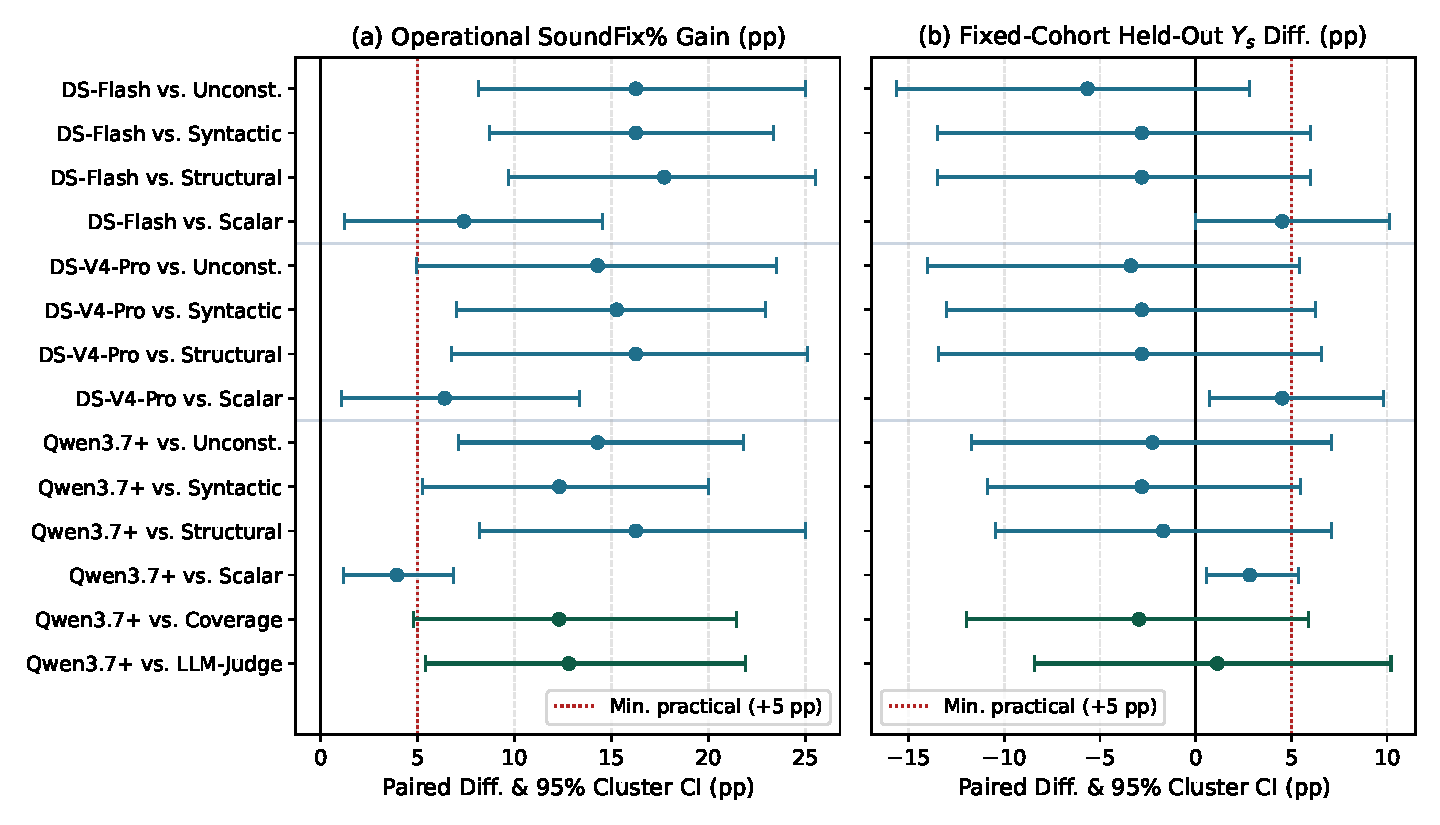
\includegraphics[width=0.96\textwidth]{figures/fig2_round_trajectories.pdf}
\caption{Whole-project clustered paired differences and 95\% confidence intervals for \textsc{MuGuard-Flake} on (a) operational sound-fix yield and (b) fixed-cohort held-out yield.}
\label{fig:forest_effects}
\end{figure*}

\paragraph{Causal Isolation of Surviving-Mutant Witnesses.}
The prefix-forked experiment across all $\ForkTotal$ frozen erosion states in $\ForkProjects$ repositories confirms that localized witnesses drive substantial recovery gains beyond gated retries alone (Table~\ref{tab:ablation} and Figure~\ref{fig:ablation_fork}). Supplying the True Witness package recovers \ForkAThreePct{} of eroded repairs, outperforming Scalar Ratio feedback (\ForkAOnePct{}) by 28.1 percentage points overall and by virtually the same margin under equal model weighting. This lift achieves clustered significance and holds across every model, spanning 20 points on confirmatory Qwen 3.7 Plus to 34 points on DeepSeek Flash.

Qualitative inspection of recovered trajectories explains why bare scalar ratios lag so sharply behind concrete witnesses. Told only that a few mutants survived, models often guess blindly, adding redundant assertions around the same weakened check or oscillating between two flaky variants. Given the exact surviving production line and source slice, by contrast, models immediately recognize the missed branch or truncated token and repair the root cause in a single follow-up turn.

\begin{table}[t]
\centering
\scriptsize
\setlength{\tabcolsep}{1.8pt}
\caption{Prefix-forked recovery from identical erosion states across all $\ForkTotal$ forks in $\ForkProjects$ repositories (100\% completed across all four arms).}
\label{tab:ablation}
\begin{tabular}{lrrrrr}
\toprule
Feedback Arm or Contrast & Mut. & Chars (Tok.) & Rec.\ / $n$ & Recovery\% [95\% CI] & Rds / $p$ ($p_{\text{Holm}}$) \\
\midrule
Gate-Only (Immediate Abstain) & 0.00 & 0 (0) & 0/129 & 0.00\% (def.) & --- \\
Scalar Ratio ($k/M$) & 0.00 & 530 (140) & 55/129 & 42.64\% [19.9, 70.3] & 1.25 \\
Misleading Witness (Stress) & 2.46 & 1901 (500) & 42/129 & 32.56\% [18.3, 52.7] & 1.50 \\
\textbf{True Witness (MuGuard)} & 2.46 & 1905 (501) & 91/129 & 70.54\% [53.4, 87.3] & 1.44 \\
\midrule
DS-Flash (True $-$ Scalar) & --- & --- & 33 vs.\ 18/44 & +34.09 [+9.09, +58.82] pp & 0.0625 \\
DS-V4-Pro (True $-$ Scalar) & --- & --- & 34 vs.\ 21/45 & +28.89 [+6.25, +52.83] pp & 0.0625 \\
Qwen3.7+ (True $-$ Scalar) & --- & --- & 24 vs.\ 16/40 & +20.00 [+8.70, +32.43] pp & 0.0312 \\
\midrule
\textbf{Pooled (True $-$ Scalar)} & --- & --- & 91 vs.\ 55/129 & \textbf{+27.91 [+11.70, +43.33] pp} & \textbf{0.0049 (0.0049)} \\
\textbf{Equal-Model (True $-$ Scalar)} & --- & --- & 3 models equal & \textbf{+27.66 [+11.80, +43.29] pp} & \textbf{0.0039} \\
\textbf{Pooled (True $-$ Misleading)} & --- & --- & 91 vs.\ 42/129 & \textbf{+37.98 [+24.32, +48.73] pp} & \textbf{0.0002 (0.0005)} \\
\bottomrule
\end{tabular}
\end{table}


The Misleading Witness arm confirms that diagnostic accuracy, not prompt verbosity, explains this gain. Keeping prompt structure and mutant count identical and pointing to already-killed mutants drops recovery to \ForkATwoPct{}, a 37.1-point deficit below True Witness on matched forks (Figure~\ref{fig:ablation_fork}). Models follow the misleading hint into irrelevant code regions, proving that mislocalized diagnostics actively harm recovery. Because roughly three-quarters of tests never trigger an erosion retry, that 28-point conditional lift translates into consistent full-cohort gains over Scalar Gate of 4 to 7 points in operational yield and 3 to 5 points in held-out yield (Figure~\ref{fig:forest_effects}). Gate enforcement and witness diagnostics thus play distinct, complementary roles: the gate stops silent erosion, and localized witnesses turn rejected drafts into valid fixes.

\begin{figure}[t]
\centering
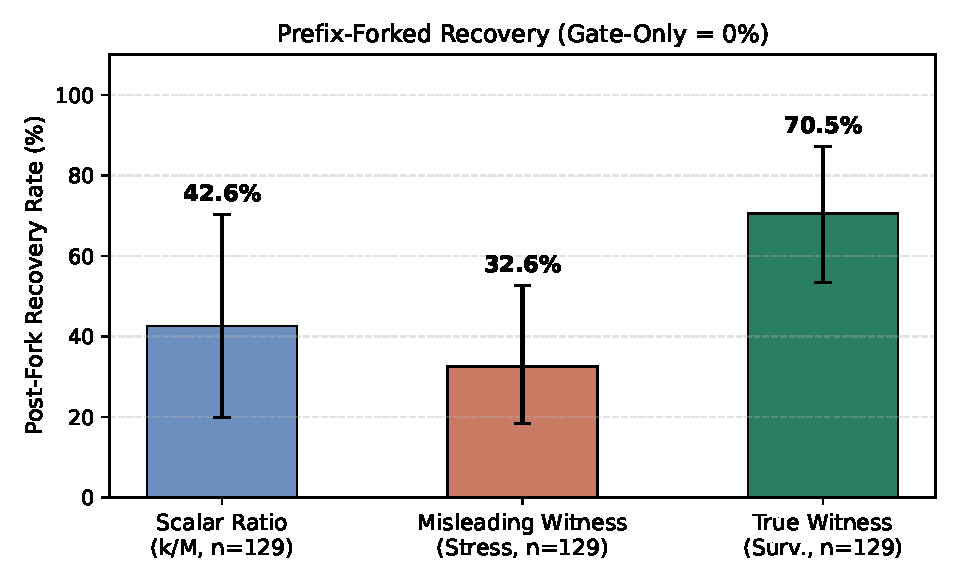
\includegraphics[width=0.74\textwidth]{figures/fig4_n14_ablation_and_pareto.pdf}
\caption{Post-fork recovery rates and 95\% cluster confidence intervals across feedback arms on frozen erosion states.}
\label{fig:ablation_fork}
\end{figure}

\medskip
\noindent\fbox{\parbox{0.97\textwidth}{\textbf{Summary for RQ3:} \textsc{MuGuard-Flake} eliminates in-loop erosion, raises operational sound-fix yield by 12 to 18 points over static guards, and cuts unseen held-out loss among accepted patches by 45\% to 65\%. Conservative abstention leaves unconditional held-out yield inconclusive, yet break-even analysis favors gating over non-mutation baselines whenever a silent regression costs more than 1.3 to 2.4 times an abstention review. Across $\ForkTotal$ prefix-forked states, localized witnesses outperform scalar feedback by 28 points.}}
\medskip

Having established the safety--coverage trade-off and witness mechanism in RQ3, RQ4 evaluates whether local mutation probing fits within practical CI latency budgets and what drives terminal abstentions.

\subsection{RQ4: Uncached Latencies, Abstentions, and Subset Sensitivity}
\label{sec:rq4}

\paragraph{Uncached Verification Latency vs.\ LLM Reasoning Cost.}
Local focal mutation probing is not the interactive bottleneck in automated flaky test repair (Table~\ref{tab:latency}). Even without caching, target mutation probing completes in a median of \LatUncachedJavaMutMed\,s on Java and \LatUncachedPyMutMed\,s on Python. Shared-scope partner probing adds 5.6\,s median in Java and 2.1\,s in Python.

Python's online gate runs more than three times faster than its single-run baseline sweep in Table~\ref{tab:benchmark} because the two stages probe different mutant sets. Offline baseline construction sweeps the full focal pool $M_{\text{focal}}$, including unkilled AST mutants and state-setter replays on OD-brittle tests. In-loop gating replays only the smaller frozen obligation subset $M_{\text{det}}$ (median 14 mutants) under standalone execution $e_{\text{iso}}$. In Java, PIT instruments covered focal classes as a unit on every invocation, keeping baseline and in-loop medians close.

By contrast, model inference dominates end-to-end repair time. Excluding network retry backoff, a single LLM reasoning call alone consumes a median of 53 to 80\,s across models. Including validation and retry rounds, end-to-end \textsc{MuGuard-Flake} sessions reach a median of 60\,s on DeepSeek Flash, 120\,s on DeepSeek V4 Pro, and 143\,s on Qwen 3.7 Plus. Within single-module CI builds, seconds-scale focal probing therefore adds only modest overhead on top of LLM generation, and short-circuiting compile or stability failures keeps probing focused strictly on viable candidates.

\begin{table}[t]
\centering
\scriptsize
\setlength{\tabcolsep}{4.0pt}
\caption{One-time $3\times$ baseline pre-computation times and uncached per-round validation stage latencies across Java and Python.}
\label{tab:latency}
\begin{tabular}{llrrrr}
\toprule
Phase & Stage / Scope & $n$ & Median (s) & IQR [P25, P75] (s) & P90 (s) \\
\midrule
Offline Pre-Comp.\ ($3\times M_{\text{focal}}$) & Java Default Mutators & 110 & 30.56 & [21.19, 42.44] & 60.30 \\
Offline Pre-Comp.\ ($3\times M_{\text{focal}}$) & Java Default+$M_{\text{ext}}$ & 110 & 39.39 & [22.39, 85.91] & 154.49 \\
Offline Pre-Comp.\ ($3\times M_{\text{focal}}$) & Python Baseline Pool & 93 & 37.10 & [23.46, 46.69] & 60.75 \\
\midrule
In-Loop Uncached (Java) & Compile & 960 & 4.07 & [2.47, 7.75] & 9.32 \\
In-Loop Uncached (Java) & Stability Reruns ($W^+$) & 891 & 4.21 & [1.95, 8.41] & 9.77 \\
In-Loop Uncached (Java) & Target Gate ($M_{\text{det}}$) & 716 & 9.51 & [6.16, 14.36] & 16.56 \\
In-Loop Uncached (Java) & Partner Gate ($M_{\text{det}}$) & 140 & 5.58 & [4.71, 5.90] & 6.34 \\
\midrule
In-Loop Uncached (Python) & Syntax Check & 219 & 0.01 & [0.01, 0.01] & 0.01 \\
In-Loop Uncached (Python) & Stability Reruns ($W^+$) & 669 & 1.00 & [0.95, 1.29] & 1.45 \\
In-Loop Uncached (Python) & Target Gate ($M_{\text{det}}$) & 495 & 3.72 & [2.64, 6.88] & 9.88 \\
In-Loop Uncached (Python) & Partner Gate ($M_{\text{det}}$) & 148 & 2.12 & [1.22, 2.98] & 4.57 \\
\bottomrule
\end{tabular}
\par\smallskip\parbox{0.96\textwidth}{\scriptsize\textit{Note:} Python in-loop gating replays only frozen killed obligations $M_{\text{det}}$ (median 14 mutants) under standalone $e_{\text{iso}}$, explaining its $3.3\times$ speedup relative to single-run full $M_{\text{focal}}$ baseline sweeps (12.29\,s in Table~\ref{tab:benchmark}; $3\times$ = 37.10\,s). Java PIT instruments covered classes per run, keeping baseline (10.21\,s) and in-loop (9.51\,s) medians close.}
\end{table}


\paragraph{Abstention Root Causes and Offline Subset Sensitivity.}
Unrecoverable oracle erosion accounts for only a minority of \textsc{MuGuard-Flake}'s terminal abstentions across the three multi-round models (25 on Flash, 28 on Pro, and 42 on Qwen). Across backbones, only five to nine tests end in erosion abstention, alongside two or three cases blocked by missing partner baseline coverage. Most abstentions stem instead from model formatting and stability limits, with malformed-patch sanity rejections and unstable reruns forming the bulk of terminal abstentions.

Inspecting those sanity rejections reveals a straightforward engineering root cause rather than an inherent flaw of mutation gating. In Python repositories, language models frequently emit class test methods with mismatched leading indentation, triggering immediate syntax rejection before stability or mutation checks even execute. Enforcing syntax-constrained decoding or deterministic method re-indentation would therefore recover substantial auto-merge coverage without weakening oracle protection.

Offline subset-sampling bounds across all \TaxUniquePatches{} unique eroded patches confirm two practical guidelines for gate configuration (Table~\ref{tab:topk} and Figure~\ref{fig:latency_topk}). First, omitting partner obligations caps maximum detection recall at 99.0\% even when probing all target mutants, because four eroded patches weaken exclusively partner obligations. Second, probing small subsets misses substantial erosion: uniform random sampling detects only 50.8\% of eroded patches at a 5-mutant budget and 68.9\% at 10 mutants, reaching 92.3\% at 25 mutants and outperforming line-dispersion and operator-priority heuristics at higher budgets.

\begin{table}[t]
\centering
\scriptsize
\setlength{\tabcolsep}{6.0pt}
\caption{Offline mutant subset-sampling detection recall across $\TaxUniquePatches$ unique eroded patches over joint target-and-partner obligation pools versus target-only probing.}
\label{tab:topk}
\begin{tabular}{lrrrrr}
\toprule
Sampling Budget & Pool Share & Uniform Random & File/Line Disp. & Operator Priority & Target-Only \\
\midrule
Top-1 & 5.1\% & 18.8\% & 19.5\% & 25.8\% & 20.7\% \\
Top-5 & 25.6\% & 50.8\% & 41.5\% & 42.8\% & 57.6\% \\
Top-10 & 44.6\% & 68.9\% & 64.2\% & 44.2\% & 75.5\% \\
Top-25 & 72.4\% & 92.3\% & 79.5\% & 84.0\% & 93.5\% \\
All & 100.0\% & 100.0\% & 100.0\% & 100.0\% & 99.0\% \\
\bottomrule
\end{tabular}
\par\smallskip\parbox{0.96\textwidth}{\scriptsize\textit{Note:} Target-Only omits partner obligations $M_{\text{det}}(T_{\text{part}})$, capping recall at 99.0\% because four eroded patches weaken exclusively partner obligations.}
\end{table}


That ordering reflects how behavioral erosion spreads across a repository. Heuristics that concentrate on a few lines or operator classes overlook faults in untouched helper methods, fixture branches, or partner classes, whereas uniform sampling covers the focal footprint more evenly. Even so, sampling trades away substantial safety for only a few seconds of saved compute. Because full single-test probing already completes in a median of under ten seconds, probing the complete target-and-partner obligation pool remains the clear default for CI merge gates.

\begin{figure*}[t]
\centering
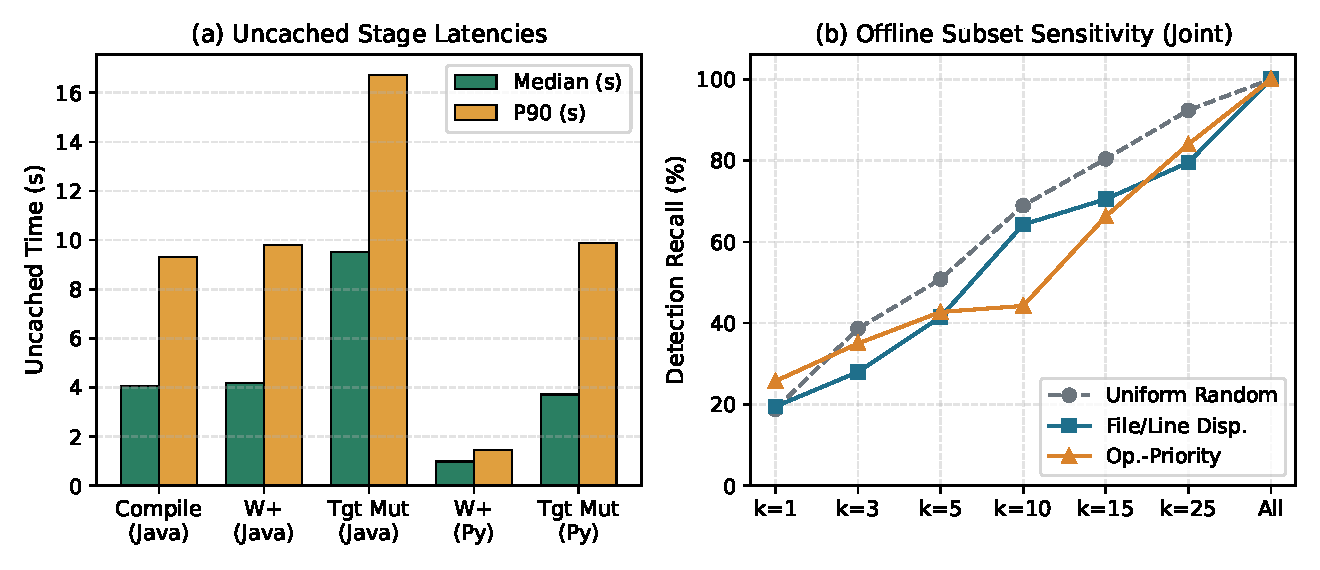
\includegraphics[width=0.95\textwidth]{figures/fig5_latency_distributions.pdf}
\caption{(a) Uncached in-loop stage latencies across Java and Python, and (b) offline subset-sampling detection recall over joint obligation pools.}
\label{fig:latency_topk}
\end{figure*}

\medskip
\noindent\fbox{\parbox{0.97\textwidth}{\textbf{Summary for RQ4:} Uncached in-loop probing takes under ten seconds median in Java and under four seconds in Python (replaying only frozen $M_{\text{det}}$ rather than full baseline $M_{\text{focal}}$), while LLM reasoning dominates session time. Most abstentions stem from Python formatting and stability limits rather than unrecoverable erosion, and full target-and-partner probing avoids both small-subset recall drops and partner-only blind spots.}}
\medskip

\section{Discussion and Practical Deployment Playbook}
\label{sec:discussion}

Rather than repeating the empirical rates from Section~\ref{sec:results}, this section translates our findings into concrete adoption decisions for continuous integration teams and methodological standards for future flaky-test benchmarks.

\subsection{Why Behavioral Verification and LLMs Act as Complements}

Our cross-language evidence explains why purely static guardrails hit a structural ceiling. Strengthening syntactic rules into assertion-correspondence heuristics still fails to predict how upstream fixture changes, delimiter normalizations, shared-state resets, or stubbed collaborators alter production execution. Worse, strict syntactic heuristics penalize legitimate structural refactorings in developer pull requests and nudge language models away from obvious assertion deletions toward subtler semantic shifts that keep every assertion call syntactically intact.

Executable probing and LLM reasoning instead solve complementary halves of the repair problem. Local mutation probing does not synthesize test code, but it supplies deterministic behavioral visibility over fixed production code. Conversely, modern LLMs excel at rewriting order-sensitive assertions once told \emph{which} production branch or side effect lost observability. The prefix-forked contrast confirms that localized counterexamples---not extra retries or longer prompts---unlock that synergy, converting rejected drafts into lossless repairs where bare numeric counts stall.

\subsection{A Practical CI Adoption and Triage Playbook}

Because strict obligation conservation trades auto-merge coverage for lower post-merge regression risk, engineering teams should treat \textsc{MuGuard-Flake} as a configurable CI safety policy rather than a one-size-fits-all switch. Three operational questions govern practical rollout:

\paragraph{1. Which Repositories Should Enable Strict Fail-Closed Gating First?}
Our asymmetric break-even analysis (Equation~\ref{eq:breakeven}) supplies an objective adoption rule: fail-closed gating achieves strictly lower expected CI cost than non-mutation baselines whenever a silently regression-blind test costs more than roughly 1.3 to 2.4 times the effort of triaging an explicit abstention ticket. Core libraries, financial or protocol serializers, shared infrastructure modules, and release-blocking CI suites sit far above that threshold and should enable strict dual-role gating by default. Conversely, fast-moving prototypes or low-criticality UI suites with scarce reviewer bandwidth may prefer an advisory mode that posts surviving witnesses as pull-request review comments without blocking merges.

\paragraph{2. When Should Teams Activate Extended Mutation Operators Beyond Defaults?}
Default bytecode and AST mutators catch all in-loop erosion and cut unseen held-out fault loss sharply at seconds-scale latency, yet our pull-request and held-out audits expose narrow semantic blind spots in encoding, URL parsing, and relational container invariants. Rather than enabling heavy operator suites globally, teams should keep default operators as the fast synchronous gate on all repositories and selectively layer extended argument-propagation or relational mutators onto security-sensitive, serialization, and protocol-encoding modules. To keep pull-request turnaround crisp, teams should trigger one-time baseline pre-computation asynchronously the moment a test is quarantined as flaky, amortizing baseline cost completely off the developer critical path.

\paragraph{3. How Should Abstention Tickets Wire Into Human Review?}
Effective human triage depends on separating avoidable formatting failures from genuine semantic trade-offs before an engineer opens a ticket. First, deterministic method re-indentation or syntax-constrained decoding should precede the repair gate in Python pipelines to eliminate formatting-driven abstentions without weakening oracle safety. Second, when the gate abstains on erosion or an uncovered partner, the CI bot should post the top surviving-mutant witnesses directly onto the pull request. Maintainers can then act in minutes by either approving a verified canonicalization override (such as deterministic serializer key sorting or intentional singleton fixture isolation) or applying a targeted fix guided by those surviving production lines. Reviewers inspecting witness-driven LLM patches should still verify intended semantics, because models can occasionally satisfy a small set of baseline return-value witnesses with shallow checks rather than exercising full domain state.

\subsection{Upgrading Empirical Standards for Flaky-Test Repair Benchmarks}

Echoing Bludau and Pretschner's call to audit proxy-induced evaluation bias~\cite{bludau2026szz} and Leunig and Petersen's industrial warning on assertion dilution~\cite{leunig2026perl}, our study suggests four concrete methodological upgrades for future flaky-test repair research:
\begin{enumerate}[nosep]
    \item \emph{Report multi-dimensional risk--coverage profiles.} Benchmarks should pair stabilization pass rates with operational soundness, conditional unseen-fault loss, fixed-cohort held-out yield, and explicit abstention counts so safety--coverage trade-offs remain transparent.
    \item \emph{Enforce exact attribution and fail-closed accounting.} Evaluators should require repeated clean baselines, exact test-case and lifecycle attribution, explicit separation of timeouts and setup errors from surviving mutants, and dual-role partner checks whenever order-dependent edits touch shared scope.
    \item \emph{Audit historical tools and developer PRs with strict provenance.} Historical baselines should filter strictly to official passing logs, developer pull requests should be applied atomically across all edited test files, and semantic diff adjudication should incorporate blinded cross-auditing with reported inter-rater reliability.
    \item \emph{Cluster inference by repository.} Because flaky tests correlate strongly within projects, future comparisons should rely on whole-repository cluster resampling and sign-flip permutation tests rather than test-level independence assumptions.
\end{enumerate}

\section{Threats to Validity}
\label{sec:threats}

Following empirical software engineering guidelines~\cite{wohlin2012experimentation,bludau2026szz}, we organize threats across construct, internal, external, and conclusion dimensions, stating both our mitigations and remaining boundaries.

\subsection{Construct Validity}

Three construct threats affect mutation-based audits of flaky test repair: \emph{Test Flimsiness}~\cite{parry2026flimsiness}, execution misattribution, and specification over-constraining. We curb flimsiness and misattribution through five-run clean baselines, focal scope restriction, exact test-case and lifecycle attribution with explicit indeterminate tracking, and three-run kill intersection, excluding five tests with fewer than three obligations. For order-dependent held-out checks, we pair repeated-pollution execution with unmodified-repository controls across all 142 order-dependent tests and keep strict yield separate from matched-control sensitivity. To prevent over-constraining from hiding behind mutation counts, we explicitly measure false rejections against audited developer pull requests.

Four construct boundaries remain. First, PIT XML output does not separate setup failures from test-body failures or record runtime exception classes, so Java held-out stratification uses mutator families rather than assertion-only runtime exceptions. Second, Python's held-out pool shares 24 mutants across sibling tests in the same repository, though never with a target test's own repair gate. Third, held-out mutants approximate regression sensitivity rather than real production bug commits~\cite{just2014mutants}. Finally, our Stage-2 blinded cross-audit using OpenAI Codex (\texttt{gpt-6-astra}, CLI v0.153.4) confirmed substantial-to-almost-perfect agreement on primary categories ($\kappa = 0.63$ to $0.83$), with all 35 primary-decision disagreements arbitrated. Nevertheless, an automated cross-audit replaces neither a second independent human annotator nor direct surveys of repository maintainers. In addition, the three-way boundary separating genuine degradation from responsibility shift on fixture-narrowing edits showed lower pre-arbitration agreement ($\kappa = 0.24$) despite 98.2\% agreement that those patches were non-legitimate.

\subsection{Internal Validity}

Internal threats include trajectory splicing, stale build artifacts, partial model completions, and prefix-forked execution mechanics. Whenever baseline pool updates, guard refinements, or JUnit~3 isolation fixes altered an earlier decision, all downstream rounds were re-executed end to end rather than spliced. In Java, compiled class files are cleared before test compilation and restored with preserved timestamps under per-repository locks to prevent stale builds. Automated regression checks, lifecycle-ordering verification, and live replay of all 1,243 held-out candidate patches guard these execution invariants end to end. Evaluating Structural Guard out-of-sample on confirmatory Qwen 3.7 Plus, Kimi K2.5, and GLM-5 further confirms that its blind spots are not artifacts of exploratory tuning.

Three execution boundaries warrant disclosure. In the prefix-forked experiment, Scalar Ratio and True Witness reused verified prefixes from the main campaign, and Misleading Witness ran fresh. Twelve Misleading Witness forks were omitted due to API token caps, and witness prompts varied naturally in length with focal slice size. Similarly, one eligible test on DeepSeek Flash and 15 on DeepSeek V4 Pro hit 16k reasoning-token caps; fixed-cohort and intent-to-treat rates score incomplete runs as zero, and confirmatory Qwen 3.7 Plus along with both cross-family single-pass models completed 100\% of runs. Finally, session latencies sum recorded per-round model and evaluation stage times without failed network retry backoff.

\subsection{External Validity}

Our benchmark spans $\BenchEligible$ tests across $\BenchProjects$ Java and Python repositories and five modern LLMs from four vendors, yet four boundaries limit generalization:
\begin{enumerate}[nosep]
    \item \emph{Model vendor and ecosystem concentration.} All five modern models in our controlled multi-round and single-pass evaluations (DeepSeek, Alibaba Qwen, Moonshot Kimi, and Zhipu GLM) originate from Chinese model providers, while Western frontier models appear only through historical GPT-4 artifacts in RQ1. Although erosion rates stay highly uniform across reasoning and non-reasoning architectures from four independent vendors, replicating the multi-round gate on current OpenAI, Anthropic, and Google frontier models remains an important external-validity extension.
    \item \emph{Concurrency and network flakiness.} Tests failing intermittently under isolated execution, such as thread races or socket timeouts, are excluded; gating concurrency repairs requires deterministic schedulers or mocked clocks.
    \item \emph{Build and probe ceilings.} Cohort selection enforced 120\,s module builds and 90\,s Java or 45\,s Python baseline probes, excluding monolithic builds and tests with fewer than three obligations. Scaling to large monorepos requires incremental build caching.
    \item \emph{Offline subset modeling.} Our Top-$k$ analysis models fixed eroded patches offline; deploying subset sampling inside live repair loops could alter trajectories and requires dedicated online evaluation.
\end{enumerate}

\subsection{Conclusion Validity}

Because flaky tests cluster within repositories, treating individual tests as independent understates variance. Every primary paired difference reports 20,000-resample whole-repository cluster bootstrap confidence intervals alongside equal-repository sensitivity checks and equal-model-weighted inference on the prefix-forked ablation. Significance tests use paired project-level Rademacher sign-flip permutations with Holm--Bonferroni family control. Where confidence intervals cross zero and permutation tests are non-significant, such as overall held-out yield under both strict and stress definitions, we report the outcome as statistically inconclusive rather than inferring superiority or equivalence.

\section{Conclusion}
\label{sec:conclusion}

Automated flaky test repair pipelines are widely evaluated by single-sided stabilization reruns, yet optimizing solely for green execution invites \emph{Stabilization via Oracle Erosion}. Across $\BenchEligible$ Java and Python flaky tests in $\BenchProjects$ repositories, roughly one in five to one in four stabilization-passing patches from historical tools and five modern LLM families silently erodes baseline fault-detection obligations. Strengthening static checks into a structural correspondence guard does not close this gap: over four-fifths of eroded patches still bypass static rules through behavioral setup, delimiter, shared-scope, and call-substitution shifts, and static rejections lower out-of-sample sound-fix yield.

Across all five LLMs, \textsc{MuGuard-Flake} eliminates in-loop erosion completely. Across the three multi-round backbones, it lifts operational sound-fix yield by 12 to 18 percentage points over static guards and cuts unseen fault loss among accepted patches by 45\% to 65\%. In a controlled prefix-forked ablation, localized witnesses recover 71.1\% of eroded repairs compared with 43.0\% under bare scalar counts. These safeguards remain explicitly bounded. Conservative abstention leaves overall end-to-end held-out yield statistically inconclusive, though expected CI cost favors \textsc{MuGuard-Flake} over every non-mutation baseline whenever a silent regression costs more than 1.3 to 2.4 times an abstention review. Moreover, 20.5\% of legitimate developer pull requests trigger false rejections, and subtle weakenings outside default mutators can still slip through. Even so, with uncached focal probing under ten seconds in Java and four seconds in Python, fail-closed mutation gating paired with explicit abstention and witness-guided review offers a practical, auditable safety gate for continuous integration.

\section*{Declarations}

\paragraph{Funding.}
No external funding was received for conducting this study.

\paragraph{Data Availability Statement.}
The complete replication package, including the frozen experimental protocol, benchmark and held-out obligation definitions, historical artifact and pull-request manifests, blinded dual-auditor reliability and arbitration records, multi-model execution traces, automated verification suites, and figure-generation scripts, is publicly available at \url{https://github.com/789748456v/MuGuard-Flake-SQJ}.

\paragraph{Competing Interests.}
The authors declare that they have no competing financial or non-financial interests relevant to the content of this article.

\paragraph{Author Contributions.}
Zhijie Li led study conceptualization, methodology design, implementation, empirical evaluation, and manuscript drafting. Ketong Liu, Shaoyang Xu, Shibo Meng, and Feiran Gao contributed to data curation, experimental validation, analysis, and manuscript review and editing. Yuli Zhao supervised the study, provided methodological guidance, and reviewed and edited the manuscript. All authors read and approved the final version.


\bibliographystyle{abbrvnat}
\bibliography{references}

\end{document}
